% !TEX TS-program = pdflatex
% !TEX encoding = UTF-8 Unicode
% arara: pdflatex: { draft: true }
% arara: biber
% arara: pdflatex: { synctex: true }
% arara: pdflatex: { synctex: true }

\documentclass[11pt]{article}

\usepackage[swedish,english]{babel} % Enables swedish typesetting, needs to be at top of document
\usepackage[utf8]{inputenc} % set input encoding (not needed with XeLaTeX
\usepackage{textcomp} % Suppress unicode char error
\usepackage{enumitem} % resume numbering in enumerations and customize list appearence
\usepackage[bottom = 110pt]{geometry} % to change the page dimensions
\geometry{a4paper} % paper format, could also be placed in documentclass options
\usepackage{graphicx} % support the \includegraphics command and options
\usepackage{pgfplots} % charts and graphs
\pgfplotsset{compat=1.8} % Avoid running in backwards compatibility mode (unsuitable tick labels; missing features)
\usepackage[parfill]{parskip} % Begin paragraphs with an empty line rather than an indent
\usepackage{verbatim} % adds environment for commenting out blocks of text & for better verbatim
\usepackage{verbdef} % inline verbatim
%\usepackage{titling} % required for setlength droptitle (below)
%\setlength{\droptitle}{-70pt} % Adjust title height
\usepackage{fancyhdr} % This should be set AFTER setting up the page geometry
\pagestyle{fancy} % options: empty , plain , fancy
\renewcommand{\headrulewidth}{0pt} % customise the layout...
\lhead{}\chead{}\rhead{} % fancyhdr style reset for header
\lfoot{}\cfoot{\thepage}\rfoot{} % fancyhdr style reset for footer
\usepackage{sectsty} % Section title
\allsectionsfont{\sffamily\mdseries\upshape} % Section font
\usepackage[backend=biber,sorting=none]{biblatex}
\bibliography{references.bib}
\usepackage{url}
\usepackage{hyperref} % href
\usepackage{nameref} % Enable referring to the actual name of the chapter
\usepackage{glossaries}
\makeglossaries

\title{Rationales and Approaches for Automated Testing of JavaScript and Standard ML}
\author{Emil Wall}
%\date{} % Uncomment to hide date, or provide a date to display

\newglossaryentry{dom}{name={DOM}, description={The Document Object Model (DOM) is a model for the content, structure and style of documents \cite{W3CDOM}. It can be seen as the tree structure of elements that HTML code consists of. A common use of JavaScript is DOM manipulation, which means dynamically changing attributes and style of the elements, or adding and removing (groups of) elements}, first={The Document Object Model (DOM)}, long={The Document Object Model}}

\newglossaryentry{js}{name={JS}, description={JavaScript (JS) is a scripting language primarily used in web browsers to perform client-side actions not feasible through plain HTML and CSS. It is formally defined in the ECMAScript Language Specification (5.1 version) \cite{ECMAScriptSpecification}, ISO/IEC 16262:2011}, first={JavaScript (JS)}, long={JavaScript}}

\newglossaryentry{sml}{name={SML}, description={Standard ML (SML) is a functional language that performs type inference at compile time and has few mutable state features, used primarily in computer science and mathematical research. SML is formally specified in The Definition of Standard ML \cite{DefinitionStandardML}}, first={Standard ML (SML)}, long={Standard ML}}

\newglossaryentry{testing}{name={Testing}, text={testing}, description={Defined here as automated software testing, unless otherwise specified. Manual testing and most forms of acceptance testing is outside the scope of this thesis}}

\begin{document}

%\pagenumbering{gobble} % Turn off page numbering

\maketitle

\vspace{100pt}
The final version will have title page and endpaper generated from \\
\url{http://pdf.teknik.uu.se/pdf/exjobbsframsida.php} and \\
\url{http://pdf.teknik.uu.se/pdf/abstract.php}. \\
Hence, this page and the abstract are temporary, to be replaced in the final version.

\newpage
\null
\newpage

\begin{abstract}
The ever increasing complexity of web applications has brought new demands on automated testing of client side JavaScript. Test-driven development of such applications depends on careful design considerations, selection of tools and frameworks and a favourable testing culture. A contrasting area is that of testing Standard ML, which is also a functional language but with some important differences, notably the static type system and immutability. % embracing a favourable testing culture

The goal with this thesis was to investigate the main problems with testing behaviour of applications written in these two programming languages, and how these problems relate to development tools and practises. What are the testability issues? Which considerations are needed in order to write stable and maintainable tests? How does testing culture affect productivity and quality of software?

Through quantitative interviews, implementation of the DescribeSML testing framework and development of tests in different settings, answers to these questions was sought. Orthogonal challenges for successful testing were identified, combined with inevitably ever present tradeoffs between rigour and simplicity. Recent advancements of technology and frameworks has meant reduced technical limitations whilst demands on software engineering excellence has remained constant if not growing. The main issues are dependency management, how to test graphical interfaces, maintaining separation of concepts, and using the right tools. Harnessing the advancements and applying pragmatism, ingenuity and persistence are key to overcoming these challenges.
\end{abstract}

\newpage
\null
\newpage

\section*{Populärvetenskaplig sammanfattning}

När en webbsida skapas så innebär det ofta flera månader av kodande innan den kan börja användas, i vissa fall flera år. Ju mer avancerad funktionalitet sidan har desto mer tid tenderar utvecklingen att ta i anspråk och desto större blir risken för buggar, särskilt om det är många personer som arbetar med sidan. När sidan väl är lanserad så återstår vanligen en ännu längre tid av drift och underhåll. I det skedet upptäcks och åtgärdas de eventuella buggar som inte hann upptäckas under utvecklingsfasen och det tenderar att ske omfattande förändringar. Det kan vara en stor utmaning att göra detta utan att introducera nya buggar eller förstöra andra delar av sidan, och förändringarna tar ofta längre tid att genomföra än man tror.

En webbsidas skick kan idag vara avgörande för om det uppstår ett förtroende gentemot ett företag, eftersom den ofta utgör ett första intryck. Vissa företag sköter även en stor del av sin centrala verksamhet genom webbsidor så om en sida inte fungerar kan till exempel beställningar eller annan information gå förlorad. Företag kan alltså få både ökade kostnader och förlorad inkomst av buggar, vilket är varför det behövs noggrannt förebyggande arbete.

Ett av de vanligaste sätten att minimera förekomsten av buggar är testning. En variant är att manuellt kontrollera funktioner, till exempel genom att lägga upp varje ny version av en sida på en testserver där man klickar sig runt på webbsidan och kontrollerar att saker fungerar som de ska innan man laddar upp den så att allmänheten kommer åt den. Detta är en billig metod på kort sikt, men det innebär ständig upprepning av tidskrävande procedurer så det kan visa sig ohållbart på längre sikt. Det medför även behov av manuell felsökning för att ta reda på varför något inte fungerar och det kan vara svårt att veta hur något är tänkt att fungera om kraven inte är tillräckligt formaliserade.

Ett alternativ är automatiserade tester, som kan testa specifika delar av koden eller simulera en användares beteende utan mänsklig inblandning. Det är den typen av tester som den här uppsatsen fokuserar på. Mycket av den teknik som används för att skapa hemsidor är förhållandevis ny och det tillkommer hela tiden nya sätt att arbeta på, så det finns ett stort behov av översikt och utvärdering av teknologin. Det finns även mycket att lära genom att jämföra denna teknik med testning i andra sammanhang och i programmeringsspråk som normalt inte används för webben. En fullständig kartläggning av alla tekniker som går att koppla till testning av webbsidor vore dock ett alltför stort projekt för detta format, så denna uppsats är avgränsad till att endast behandla JavaScript och Standard ML, två programmeringsspråk med intressanta likheter och skillnader.

JavaScript används inom webbutveckling för att skapa interaktiva sidor med minimal trafik mot servrar. Standard ML å andra sidan är uppbyggt annorlunda och används oftast i helt andra sammanhang, men stödjer i grunden en liknande programmeringsstil. Det har den senaste tiden skett framsteg inom testning för dessa programmeringsspråk, mycket tack vare att information om hur man går tillväga har blivit mer tillgänglig, nya ramverk gör att kod struktureras på ett annat sätt än tidigare och det har uppstått fler och stabilare sätt att köra koden på. Här ges en överblick över dessa framsteg, och de många tekniker som idag används för testdriven utveckling.

Genom egen utveckling och intervjuer med andra utvecklare har problem och lösningar inom området undersökts. Några av de större svårigheter som identifierats är att vissa mekanismer (asynkront beteende, DOM-manipulation, grafiska komponenter) är svåra att testa utförligt utan att testerna blir opålitliga eller långsamma, att det sällan lönar sig att skriva tester i efterhand, att det kan vara svårt att hålla tester lättförståeliga och uppdaterade, att utvecklingsverktygen kan vara begränsande, och att programmeringsspråkens uppbyggnad och typen av applikation har viss inverkan på vad som är möjligt och lämpligt att testa. Det spelar även stor roll vilka erfarenhetsmässiga och kulturella förutsättningar utvecklarna har för att skriva tester.

Testning i sig är inte en lösning på alla problem och olika former och nivåer av testning lämpar sig för olika situationer, men när det används rätt så kan det gynna både användare, organisationer och utvecklarna själva. En viktig slutsats är att testning behöver ses som ett verktyg och inte ett självändamål och att utvecklare behöver hitta de metoder och verktyg som fungerar bäst för dem.

\newpage

\section*{Acknowledgment}

Thanks goes to my supervisors Tobias Hasslebrant and Jimmy Larsson for providing me with valuable feedback and connections, to my reviewer Roland Bol for guiding me through the process and giving useful and constructive comments on my work, to the people I have had contact with and interviewed as part of this work, to all my wonderful colleagues at Valtech that never fail to surprise me with their helpfulness and expertise, and to my family and friends (and cats!) for all the little things that ultimately matters the most.

\newpage
\null
\newpage

\tableofcontents

\newpage

\pagenumbering{arabic} % Turn page numbering back on

\tableofcontents % Remove when uncommenting line above

\printglossaries

\newpage

\section{(ML1,JS1)Introduction}

Imagine the following scenario: You have been working for many months on a medium size web application project, with demanding technical challenges, using a framework that was previously unknown to you and with constantly changing requirements. People have come and gone from your team and there are parts of the code that no one in your team dares to modify, because no one understands it and too much of the functionality depends on it. Over time, patches and hacks have spread to all over the code base and it feels as if for every bug you fix, new ones are introduced and the complexity of the application is constantly increasing. Every few weeks you feel unbalanced and nervous about the next release, with frightful memories fresh in mind and a feeling that you should be able to do better.

Now envision this: Despite the challenging requirements and conditions, you are relatively sure that the application works as it should. You feel safe in telling the customer when a feature has been implemented because the automated tests indicate that it works and that nothing else has broken. The application has a modular design and you have a good feeling of what every part is supposed to do and how the system works as a whole. This makes it easier to implement change requests and you spend relatively little time debugging, because the tests generally give you precise indications about which parts of the code are affected by your changes. Whenever there is a bug, you capture it with tests so that you will easily notice if it is re-introduced. Releasing a new version is simple and you feel proud of being part of the team.

The main difference between these scenarios is that the second one requires a pervading \gls{testing} effort from the team. In this thesis, we will look at how to achieve this for \gls{js} and \gls{sml}. Many of the topics discussed are applicable to other programming languages as well, these were chosen because the automated testing community around \gls{js} still has some ground to cover \cite[p.~xix]{Tddjs} and for \gls{sml}, a less known functional language, the situation is even more severe. This is evident when compared to other programming communities such as Ruby and Java. As illustrated by Mark Bates \cite{TestingStatistics}:

\begin{quote}
``Around the beginning of 2012, I gave a presentation for the Boston Ruby Group, in which I asked the crowd of 100 people a few questions. I began, `Who here writes Ruby?' The entire audience raised their hands. Next I asked, `Who tests their Ruby?' Again, everyone raised their hands. `Who writes JavaScript or CoffeeScript?' Once more, 100 hands rose. My final question: `Who tests their JavaScript or CoffeeScript?' A hush fell over the crowd as a mere six hands rose. Of 100 people in that room, 94\% wrote in those languages, but didn't test their code. That number saddened me, but it didn't surprise me.''
\end{quote}

\begin{center}
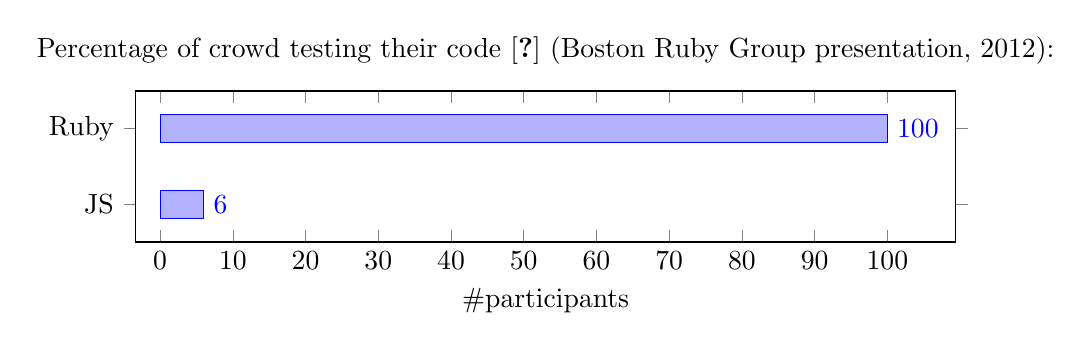
\begin{tikzpicture}
\begin{axis}[
title={Percentage of crowd testing their code \cite{TestingStatistics} (Boston Ruby Group presentation, 2012):},
xbar,
width=12cm, height=3.5cm, enlarge y limits=0.5,
xlabel={\#participants},
symbolic y coords={JS,Ruby},
ytick=data,
nodes near coords, nodes near coords align={horizontal},
]
\addplot coordinates {(6,JS) (100,Ruby)};
\end{axis}
\end{tikzpicture}
\end{center}

\subsection{(ML1,JS1)Motivation}
\label{subsec:motivation}

Why testing, you may ask. Jack Franklin, a young \gls{js} blogger from the UK, gives three reasons: it helps you to plan out your APIs, it allows you to refactor with confidence, and it helps you to discover regression bugs (i.e. when old code breaks because new code has been added). Writing tests to use a library before actually writing the library puts focus on intended usage, leading to a cleaner API. Being able to change and add code without fear of breaking something greatly accelerates productivity, especially for large applications. \cite{JackFranklin} Without tests, the ability to refactor (see section \ref{subsec:refactor}) is greatly hampered and without refactoring, making changes becomes harder over time, the code becomes harder to understand, the number of bugs increases and more time will be spent debugging \cite[p.~47-49]{Refactoring}. In order to avoid this, code should be tested, preferably writing tests first in order to guarantee testability and avoid making testing into a cumbersome task, separated from the rest of the development.

Implementations of \gls{js} differ, especially for host objects such as document and XMLHttpRequest whose semantics are not fully defined in the specification but also for native objects that may be missing or behave differently in some implementations because they were not defined in previous specifications. Automated testing can help you discover bugs that appear due to such deviant behaviour in present and future versions. \gls{js} is also particularly important to test due to its dynamic properties \cite{AutomatedTesting} that complicate static analysis (however, there are lint tools, see sections~\ref{subsec:Lint} and \ref{subsec:refactor}), unwieldy syntax and aberrant object orientation support. \gls{js} is a complex language that requires many work-arounds because of its scoping rules and other unexpected behaviour \cite[appendix A]{GoodParts}. Despite the wide variety of testing frameworks that exists for \gls{js}, it is generally considered that few developers use them and instead rely on manual testing \cite{AutomatedTesting}.

Several implementations of \gls{sml} exist and just as with \gls{js}, there are some differences between them. \gls{sml} has extensive static analysis capabilities and since side effects are relatively rare, the output of functions tends to be predictable, leading to lower complexity in many cases, at the cost of flexibility. \gls{sml} has no built in support for automated testing and there are few testing frameworks available (see section \ref{mltestingframeworks}).

More than 90 \% of today's websites use \gls{js} \cite{BusinessJavascript} and its applications have become increasingly complex \cite[question~23]{Ekelof}. \gls{sml} on the other hand, although not nearly as widespread, is used in critical applications. The potential risk of economic loss associated with untested code being put into production, due to undetected bugs, shortened product lifetime and increased costs in conjunction with further development and maintenance, constitutes the main motivation for this thesis.

For \gls{sml} programs, usage scenarios tend to be different from \gls{js} in that \gls{sml} tends to be used more for back-end logic and algorithm design than web application front-ends. \gls{sml} is well suited for formal verification, so it is sometimes used to eliminate risk of software failure. In theory this is of course excellent, but how about practical aspects such as how difficult it is to do, how much benefits there are for maintainability, modularity and code design, and how much time is consumed to perform the verification? In which scenarios is it feasible and how does it affect productivity and the ability to make large changes to the code and get quick and frequent feedback whether the program is still correct? Even though testing can seldom provide the same guarantees as formal verification, there are many scenarios in which it is more cost effective and makes life easier for the developer. The two can of course also be used in parallel.

To achieve maximal gain from testing, the tests need to be of high quality, which means that they should be maintainable and test the right thing. How to achieve this is an important part of this thesis, which is discussed in section~\ref{subsec:quality}.

Unit testing is particularly powerful when in combination with integration tests in a
\newglossaryentry{ci}{name={CI}, description={Continuous Integration (CI) is a practise based on frequently merging new code with a main code repository, commonly using principles such as automated build, testing and deployment}, first={Continuous Integration (CI)}, long={Continuous Integration}}
\gls{ci} build with \newglossaryentry{autodeploy}{name={Automated Deployment}, text={automated deployment}, description={Auto-deploy enables automatic release to test or production, possibly as part of a Continuous deployment strategy}}\gls{autodeploy}.
This enables you to harness the power of \gls{ci}, avoiding errors otherwise easily introduced as changes propagate and affect other parts of the system in an unexpected way. The integration tests will make developers aware if they are breaking previous functionality, when changing parts of the system that the \gls{js} depends upon.

Testing \gls{js} paves the way for test-driven development, which brings benefits in terms of the design becoming more refined, and increased maintainability. Tests can serve as documentation for the code and forcing it to be written in a testable manner, which in itself tends to mean adherence to principles such as separation of concerns, and single responsibility.

The goal with this thesis is to investigate why \gls{js} testing has been performed to such a small extent, and what potential implications an increased amount of testing could provide for development and business value. Providing possible approaches to testing \gls{js} under different circumstances are also part of the goal. % TODO elaborate and update

\subsection{(ML1,JS1)Background to Project}

The first known \gls{js} testing framework JsUnit\footnote{\url{https://github.com/pivotal/jsunit}} was created in 2001 by Edward Hieatt \cite{GoingFaster} and since then several other test framework has appeared such as the testing framework for jQuery, which goes under the name QUnit\footnote{\url{http://qunitjs.com/}}, and JsUnits sequel Jasmine\footnote{\url{http://pivotal.github.com/jasmine/}}. There are also tools for mocking (see section~\ref{subsec:mocking}) such as Sinon.JS\footnote{\url{http://sinonjs.org/}}. It seems as if the knowledge of how to smoothly get started, how to avoid making the tests non-stable and time consuming, and what to test, is rare. Setting up the structure needed to write tests is a threshold that most \gls{js} programmers do not overcome \cite{TestingStatistics} and thus, they lose the benefits, both short and long term, otherwise provided by testing.

There is only one production quality testing framework available for \gls{sml}, namely QCheck\footnote{\url{https://github.com/league/qcheck}}. A few others exist but have not gained any traction and are relatively small, typically less than a year old and not under active development. The recent increase in the number of testing frameworks could be a consequence of developers being more willing to share their work as open source, or an indication that testing has been increasingly popular over the last one or two years, just as in the \gls{js} community \cite[question~1]{Edelstam}. An exhaustive list of the other \gls{sml} testing frameworks and a short discussion about their differences can be found in the Appendix.
\label{mltestingframeworks}

In section \ref{subsec:patternsexamples}, it is mentioned that examples are often simple and seldom provide a full picture. In contrast, the problem domain of this thesis is to focus on how to test the behaviour of \gls{js} that manipulates \gls{dom} elements, fetches data using asynchronous calls, validates forms, communicates through APIs or manipulates the appearance of a web page. We also look at when and why you should test your \gls{js}.

\section{(ML1,JS1)Scope and Delimitations}

Since \gls{sml} has a smaller user base than \gls{js}, much of the research has been focused on \gls{js}. Researching today's limited testing of \gls{js} may be done from a multiple different points of view. There are soft aspects such as:
\begin{itemize}[label={--}]
\item Differences in attitudes towards testing between different communities and professional groups and knowledge about testing among \gls{js} developers (section~\ref{sec:testingculture})
\item How \gls{js} is typically conceived as a language and how it is used (section~\ref{ssubsec:interviewees})
\item Economic viability and risk awareness (section~\ref{subsec:projectrisks})
\end{itemize}

There are also more technical aspects:
\begin{itemize}[label={--}]
\item Testability of \gls{js} code written without tests in mind (section~\ref{sec:testability})
\item Usability of testing tools and frameworks (sections \ref{subsec:angularjasminekarma}, \ref{subsec:jstestdriverintegration} and \ref{subsec:jstestdriver})
\item Reasons not to include frameworks in a project for the sole purpose of facilitating testing
\item Limitations in what can be tested
\item Complexity in setting up the test environment; installing frameworks, configuring build server, exposing functions to testing but not to users in production, etc.
\end{itemize}

The scope of this thesis was to look mainly at \emph{automated} testing of \gls{sml} and \emph{client side} \gls{js}. This meant that the impact of frameworks specialised for server side \gls{js} code such as vows\footnote{\url{http://vowsjs.org/}} and cucumis\footnote{\url{https://github.com/noblesamurai/cucumis}} was not considered. Testing client side code is by no means more important than server side, but in many aspects it is different and sometimes harder.

\gls{js} testing frameworks that are no longer maintained such as JsUnit\footnote{\url{https://github.com/pivotal/jsunit}} and JSpec\footnote{\url{https://github.com/liblime/jspec}} was deliberately left out of consideration. Others were left out because of a smaller user base or lack of unique functionality; among these we find TestSwarm, YUI Yeti and RhinoUnit. These are useful tools but since they are so many it would not have been realistic to include them all.

The choice of looking at \gls{sml} and \gls{js} specifically was based on that they both have problems with testing culture, but for different reasons. During preliminary studies, many people seemed concerned about how to test \gls{js}, so looking into it seemed like a good idea. The main reason to also look at testing of \gls{sml} was that there was previously no BDD framework available for it, and that it is a functional language just like \gls{js}, but typically used differently.

Manual testing was not covered to any significant extent, since there were enough issues to deal with in automated testing. Naturally, there are many situations where manual testing is required, but in this thesis \emph{testing} typically refers to automated testing.

\subsection{(,)Consequences of JavaScript testing}

There are consequences (good and bad) of testing \gls{js} both from a short and from a longer perspective. The development process is affected; through time spent thinking about and writing tests, shorter feedback loops, executable documentation and new ways of communicating requirements with customers. The the quality and maintainability of the end result is also likely to be positively affected. Making changes becomes easier when the application is supported by a rigorous set of tests, so ideally, the pace of development does not stagnate. The extra time required to set up the test environment and write the actual tests may or may not turn out to pay off, depending on how the application will be used and maintained.

\subsection{(,)Covering Common and Advanced Cases}

Accounting for how to conveniently proceed with \gls{js} testing should cover not only the simplest cases but also the most common and the hardest ones, preferably while also providing evaluation and introduction to available tools and frameworks. Many introductions and tutorials found for the testing frameworks today tends to focus on the simple cases of testing, possibly because making an impression that the framework is simple to use has been more highly prioritised than covering different edge cases of how it can be used that might not be relevant to that many anyway. To provide valuable guidance in how to set up a testing environment and how to write the tests, attention must be paid to the varying needs of different kinds of applications. It is also important to keep in mind that the tests should be as maintainable as the system under test, to minimise maintenance costs and maximise gain.

\section{(,)Technical Background}

This section gives an overview of concepts and tools relevant to understanding this thesis. Readers with significant prior knowledge about web development and \gls{js} testing may skip this section.

\subsection{(,)Basics of Testing}

Every developer performs testing in one way or another. Running an application, interacting with it and observing the results is one form of testing. The more time spent on developing the application, the more evident the need for automated tests tends to become, to reduce the amount of manual work and time spent repeating the same procedures.

Automated testing is commonly divided into different categories of tests, that exercise the code in different ways and for different reasons. Unit testing and integration testing is perhaps the most common concepts. Unit testing focuses on testing units (parts) of an application, in isolation from the rest of the application, whereas integration testing is about testing that the units fit together. Sometimes there is an overlap between the concepts, where a unit is relatively large.

Commonly, unit tests are more low level and integration tests are more like user interactions. This does not have to be the case however, unit tests can be written in a business value focused fashion too and integration tests can usually be written before there is a GUI to interact with. \cite[question~20]{Ahnve}

\subsection{(,)Behaviour-Driven Development}

Behaviour-Driven Development (BDD) is about describing expected behaviour of systems and writing tests from the outside in. It replaces and adds terminology traditionally used within TDD and encourages descriptive naming of tests (often referred to as specs, which is short for specifications, in BDD) that helps readability and to make failure messages more helpful. \cite[questions~17-18]{Ahnve}

Another advantage with BDD is the Given, When, Then (GWT) form (which is also mentioned in section \ref{subsec:tools}). It provides a context for the specs and can help in avoiding having a single setup for all tests of a specific class, which is otherwise common in classical TDD in languages such as Java. Having a single setup can be problematic because it creates dependencies between tests and can make them harder to understand. A common alternative to the GWT form is nested describe clauses with it-specs as in Jasmine and BDD style mocha. This requires more discipline from the developer because the context has to be covered by the describe text. \cite[question~19]{Ahnve}

Strictly speaking, you do not need a BDD framework to perform BDD. J. B. Rainsberger, the author of JUnit Recipes: Practical Methods for Programmer Testing, explained how to do BDD in jUnit at the XP 2011 conference in Madrid. The key to doing this is to divide the tests based on system behaviour rather than classes. This is the same concept as when writing specs in Cucumber, a Ruby GWT framework, and the same principle applies to BDD in \gls{js}. This is desirable because it helps you to not prioritise implementation details in favour of the parts that truly matters from a business value point of view.\cite[question~20]{Ahnve}

\subsection{(,)Lint Tools for JavaScript}
\label{subsec:Lint}

Linting is a static analysis tool for detecting syntax errors, risky programming styles and failure to comply to coding conventions. There are lint tools available for \gls{js} such as JSLint, JSHint, JavaScript Lint, JSure, the Closure compiler and PHP CodeSniffer. JSLint does provide some help to avoid common programming mistakes, but does not perform flow analysis \cite{JSLint} and type checking as a fully featured compiler would do, rendering proper testing routines the appropriate measure against programming mistakes.

\subsection{(,)Mocking and Stubbing}
\label{subsec:mocking}

Mocking and stubbing involves simulation of behaviour of real objects in order to isolate the system under test from external dependencies. This is typically done in order to improve error localisation and execution time, and to avoid unwanted side-effects and dependencies such as communication with databases, across networks or with a file system \cite[ch.~2]{Legacy}. A mock is different from a stub in that it has pre-programmed expectations and built-in behaviour verification \cite[p.~453]{Tddjs}.

In \gls{js}, tools for stubbing can be superfluous because you are able to manually replace functions with custom anonymous functions, that can have attributes for call assertion purposes. The stubbed functions can be stored in local variables in the tests and restored during teardown. This is what some refer to as VanillaJS \cite[question~53]{Edelstam}. It might come across as manual work that you can avoid by using a stubbing tool, but the benefits include fewer dependencies and sometimes more readable code, as mentioned in section \ref{LiteralFakes} \cite[questions~54-55]{Edelstam}. However, bear in mind that since \gls{js} has no notion of interfaces, it is easy to accidentally use the wrong method name or argument order when stubbing a function \cite[p.~471]{Tddjs}.

Typical cases for using a stubbing or mocking framework rather than VanillaJS include when your assertion framework has support for it, as is the case for Jasmine, when you feel the need to do a complex call assertion, mock a large API or state expectations up front as is done with mocks. Bear in mind that overly complex stubbing needs can be a symptom for that the code is in need of refactoring \cite[question~34]{Stenmark}, and strive for consistency by using a single method for stubbing -- mixing VanillaJS with Jasmine spies and Sinon.JS stubs will make the tests harder to understand.

\subsection{(,)Browser Automation}
\label{subsec:browserautomation}

Repetitive manual navigation of a web site is generally boring and time consuming. There are situations where manual testing is the right thing to do, such as when there is no need for regression testing or the functionality is too complicated to interact with for automated tests to be possible (but then the design should probably be improved). Most of the time, tasks can be automated. There are several tools available for automating a web browser: the popular open source Selenium WebDriver, the versatile but proprietary and windows specific TestComplete and Ranorex, the Ruby library Watir and its .NET counterpart WatiN, and others such as Sahi and Windmill.

Selenium WebDriver is a collection of language specific bindings to drive a browser, which includes an implementation of the W3C WebDriver specification. It is based on Selenium RC, which is a deprecated technology for controlling browsers using a remote control server. A common way of using Selenium WebDriver is for user interface and integration testing, by instantiating a browser specific driver, using it to navigate to a page, interacting with it using element selectors, key events and clicks, and then inspecting the result through assertions. These actions can be performed in common unit testing frameworks in Java, C\nolinebreak\hspace{-.05em}\raisebox{.3ex}{\scriptsize\bf \#}, Ruby and Python through library support that uses the Selenium Webdriver API. \cite{Selenium}

There is also a Firefox plugin called Selenium IDE, that allows the user to record interactions and generate code for them that can be used to repeat the procedure or as a starting point in tests. In the remaining parts of this thesis, we will mean Selenium WebDriver when we say Selenium, and refer to Selenium IDE by its full name.

\subsection{(,)Refactoring}
\label{subsec:refactor}

Refactoring is ``a change made to the internal structure of software to make it easier to understand and cheaper to modify without changing its observable behaviour'', or the act of applying such changes \cite[p.~46]{Refactoring}. As mentioned in the \nameref{subsec:motivation} section (section \ref{subsec:motivation}), refactoring prevents program decay and helps to maintain productivity. Just like testing, refactoring is no magic bullet that solves all problems and it is important to know when to do it and when it might not be worth the effort. Common rules of thumb are to refactor when doing something similar for the third time (a pragmatic approach to the DRY principle), when it helps to understand a piece of code, when it facilitates addition of a new feature, when searching for a bug and when discussing the code with others, e.g. in code reviews \cite[p.~49-51]{Refactoring}.

Using refactoring tools can be very helpful to see which parts of the code is in most need of refactoring, and to automate certain refactoring actions by facilitating renaming, method extraction, etc. \cite[ch.~5]{Legacy}. There is some support in IDEs such as Visual Studio (using
JSLint.VS\footnote{\url{http://jslint.codeplex.com/}},
ReSharper\footnote{\url{http://www.jetbrains.com/resharper/}} and/or
CodeRush\footnote{\url{http://www.devexpress.com/Products/CodeRush/}}),
WebStorm IDE\footnote{\url{http://www.jetbrains.com/webstorm/features}} (or
IntelliJ Idea\footnote{\url{http://www.jetbrains.com/editors/javascript_editor.jsp?ide=idea}} using a plugin) and
NetBeans\footnote{\url{https://netbeans.org/kb/docs/ide/javascript-editor.html}}. There are also standalone statistical tools such as
kratko.js\footnote{\url{https://github.com/kangax/kratko.js}} and
jsmeter\footnote{\url{https://code.google.com/p/jsmeter/}} (not to be confused with the
Microsoft Research project\footnote{\url{http://research.microsoft.com/en-us/projects/jsmeter/}}) that helps you to identify which objects have too many methods and which methods do too many things (or have too many arguments). Relying on metrics such as lines of code is of course not always appropriate due to different coding styles, but at least it provides an overall picture \cite{Kratko}.

\subsection{(,)Build tools}
\label{subsec:build}

There exists some general build tools that can be used for any programming language, these are often installed on build servers and integrated with version control systems. Examples include Jenkins, which is often configured and controlled through its web interface although it also has a CLI, and GNU Make, which is typically configured using makefiles and controlled through CLI. In addition to these, there are also language specific tools: Ruby has Rake, Java has Maven, Gradle and Ant, C\nolinebreak\hspace{-.05em}\raisebox{.3ex}{\scriptsize\bf \#} has MSBuild and NAnt.

Naturally, there are build tools designed specifically for \gls{js} as well, Grunt\footnote{\url{http://gruntjs.com/}} being the most popular, which can be installed as a node.js package, has plugins for common tasks such as lint, testing and minification, and can be invoked through CLI. \cite[question~52]{Edelstam} Jake and Mimosa are other well known and maintained alternatives. It is also possible to use Rake, Ant or similar. Just as JsTestDriver and Mocha have adapters for Karma and Jasmine (see section~\ref{subsec:frameworks}), Rake has evergreen\footnote{\url{https://github.com/jnicklas/evergreen}} that allows it to run Jasmine unit tests. \cite{BuildTools}\cite[question~6]{Ahnve}

\subsection{(,)Setting up a test suite}

Many people have never set up a testing framework in a project and thinks that it is a hard thing to do. It is typically not, unless you want to do something very special such as automatic test generation or integration with a service of some sort. However, it is worth giving careful thought on what combination of tools to use, to enable a pleasant workflow and ensuring that the tests can be written in a desirable style.

Build programs (see section~\ref{subsec:build}) and version control systems play an important role in automating testing.


\section{(,)Methods}

The methods used were first and foremost qualitative in nature, in order to prioritise insight into the problem domain above quantitatively verifying hypotheses. The chance of finding the true difficulties of \gls{js} testing was expected to increase with open questions.

The work of this thesis began with an extensive literature study and an overview of technologies and frameworks. Interviews of \gls{js} developers of different background were performed and analysed. There was also some hands on evaluation of tools and frameworks, assessment of testability and impact of adding tests to existing projects.

In order to describe ways of writing tests for \gls{js}, the practical work involved testing an existing application, performing TDD exercises from Test-driven JavaScript Development \cite{Tddjs} and doing some small TDD projects during the framework evaluation. There were plans to have a workshop field study, where programmers would work in pairs to solve pre-defined problems using TDD, but in the end it was decided that it would be too difficult to extract useful data from such an activity.

\subsection{(,)Literature Study}

Relevant books, articles and Internet sources were identified and skimmed, some were read through thoroughly. Over time, several new titles were published and some older literature was also included as the need became apparent.

\subsection{(,)Framework Overview and Evaluation}

The following testing frameworks have been evaluated:
Jasmine\footnote{\url{http://pivotal.github.com/jasmine/}} (+ Jasmine-species\footnote{\url{http://rudylattae.github.com/jasmine-species/}}),
qUnit\footnote{\url{http://qunitjs.com/}},
Karma\footnote{\url{http://karma-runner.github.io/}},
Mocha\footnote{\url{http://visionmedia.github.com/mocha/}},
JsTestDriver\footnote{\url{https://code.google.com/p/js-test-driver/}},
Buster.JS\footnote{\url{http://docs.busterjs.org/}} and
Sinon.JS\footnote{\url{http://sinonjs.org/}}. The code written while evaluating the frameworks is publicly available as git repositories under my Github account \emph{emilwall}, together with the \LaTeX~code for this report.

\subsection{(,)Interviews}

Semi-structured case study interviews were used rather than surveys to gather individual views on the subject. This approach allowed for harnessing unique as well as common experiences which would not be picked up in a standardised survey. The interviews were between 20 and 60 minutes long and were conducted both in person and via Internet video calls.

\subsubsection{(,)Interview Considerations}

The preparations before the interviews included specifying purpose and which subjects to include, select interviewees, preparing questions and adjust the material to fit each interviewee. The interviews took place rather late so that preliminary results and insights from the literature study could be used as basis for the discussions.

The purpose of the interviews was to investigate attitudes and to get a reality check on ideas that had emerged during previous work. Selecting the interviewees was to a large extent done based on availability, but care was also taken to include people outside of Valtech and to get opinions from people with different background (front-end, back-end, senior, junior, etc.). Enquires were made in Valtech's intranet, my supervisor asked his contacts via his Twitter account and I contacted some people via mail. This led to five interviews and one email conversation, which can all be found in the Appendix.

The interviews were performed in swedish to allow for a more fluent conversation and minimise risk of misunderstandings. They were transcribed (see Appendix), each question was given a number, and the most relevant parts were translated and included in this report with reference to the question numbers. The interviewees were asked prior to the interviews if it was ok to record the conversation and if they wanted to be anonymous, everyone was ok with being recorded and mentioned by name.

The interviewees received questions beforehand via mail which most of them answered before the interview. This allowed the interviews to focus on the vital parts rather than personal background and opinions about \gls{js}. The questions that was sent out before the interviews were mainly about previous experience with \gls{js} and testing, frameworks, attitudes towards the language, difficulties with testing and opinions and observations on benefits of testing.

\subsubsection{(,)The Interviewees}
\label{ssubsec:interviewees}

The first person I interviewed was Johannes Edelstam, an experienced Ruby and \gls{js} developer, organiser of the sthlm.js meet-up group, a helping hack, and a former employee of Valtech, now working at Tink. He has a positive attitude towards \gls{js} as a programming language and has extensive experience of test driven development.

Next up was Patrik Stenmark, a Ruby and \gls{js} developer since 2007. He is also an organiser of a helping hack and a current employee at Valtech. He considers \gls{js} to be inconsistent and weird in some aspects but appreciates the fact that it is available in browsers and has developed large single page applications (SPA) in it.

The third person that was interviewed was Marcus Ahnve, a senior developer and agile coach that has been in business since 1996 working for IBM, Sun Microsystems and ThoughtWorks, and as CTO for Lecando and WeMind. He is currently working at Valtech. He is an experienced speaker and a founder of Agile Sweden, an annual conference since 2008. He is also experienced with test driven development in Java, Ruby and \gls{js}.

The next interview was with Per Rovegård, a developer with a Ph.D. in Software Engineering from Blekinge Institute of Technology. He has worked for Ericsson and is currently a consultant at factor10 where he has spent the last year developing an AngularJS application, with over 3000 tests. He is the author of the programatically speaking blog and have done several talks at conferences and meet-ups, most recently about Angular and TDD at sthlm.js on the 2nd of Oct 2013 but the interviews took place in Aug over Skype.

The last interview was with Henrik Ekelöf, a front-end developer that has seven years of professional experience with \gls{js}. He has previously worked as webmaster and web developer at Statistics Sweden and SIX and is now technical consultant at Valtech. I met him in person during my introduction programme in Valtech where he had a session with us about idiomatic \gls{js}, linting and optimisations, but this interview was done over Skype since he works out of town.

\subsubsection{(,)Other People Involved}

As can be seen at the end of the Appendix, there were some email conversations with people that was not interviewed as well. Among those are: Fredrik Wendt, who is a senior developer and consultant at Squeed specialising in team coaching with coding dojos, TDD and agile methodologies. David Waller, teacher at Linnéuniversitetet in a course about Rich Internet Applications with JavaScript. Marcus Bendtsen, teacher at Linköpings Universitet in a course about Web Programming and Interactivity.

\section{(,)Previous work}

\subsection{(,)Books}

The main source of reference within the field of \gls{js} testing today is \emph{Test-Driven JavaScript Development} \cite{Tddjs} by Christian Johansen which deals with \gls{js} testing from a TDD perspective. Johansen is the creator of Sinon.JS\footnote{\url{http://sinonjs.org/}} and a contributor to a number of testing frameworks hosted in the open source community.

Lately, a large number of books about \gls{js} testing has appeared. \emph{JavaScript Testing with Jasmine} \cite{JasmineBook} covers the Jasmine testing framework in detail, \emph{Behaviour Driven Development with JavaScript} \cite{BDDJS} presents a BDD perspective of \gls{js} testing and \emph{Testable JavaScript} \cite{TestableJS} looks at testability aspects of \gls{js}. All three of these were published this year, and Johansen's book was published only a few years ago in 2010.

Except for discussions on how to perform mathematical proofs and equality tests of polymorphic types, there are no books that cover testing of \gls{sml}. The main sources of reference for \gls{sml} is \emph{The Definition of Standard ML} \cite{DefinitionStandardML} which cover the language syntax and semantics, \emph{The Standard ML Basis Manual} \cite{BasisManual} which describes the standard library, \emph{Elements of ML Programming} which \cite{ElementsML} which cover the features of \gls{sml} in a more comprehensible fashion, \emph{ML for the Working Programmer} \cite{WorkingProgrammer} which is somewhat outdated but comprehensive, and various lecture notes \cite{ProgSml97}\cite{ProgSmlHarper}\cite{FunctionalML}\cite{NotesSMLNJ}. None of these describe ways of doing automated testing and there seems to be an attitude against testing based on that it can not prove absence of errors in the way formal verification can \cite[p.~16]{ProgSmlHarper}.

\subsection{(,)Articles}

There are many academic papers about testing web applications available, and quite a few of them focus on \gls{js} specifically (whereas practically none involve \gls{sml}). Papers on testing of \gls{sml} are hard to find even outside of the web applications context, most that are of any interest are concerned with formal verification or related to the QuickCheck tool which can be used to generate tests for Haskell code, using \gls{sml} as an intermediate language.

This idea of generating tests has also been applied to \gls{sml} and \gls{js}. \emph{A Framework for Automated Testing of JavaScript Web Applications} \cite{AutomatedTesting} focus on automatically generating tests to achieve a high degree of code coverage. The problem with this is that the ability to employ test driven development is generally more valuable than high code coverage, due to its effect on the system design. Most likely, automatically generated tests tend to be harder to maintain and cause false positives as the code changes after the tests have been generated.

QuickCheck and its \gls{sml} counterpart QCheck are based on another principle than the framework presented in the paper just mentioned, they are specified in terms of properties that should hold rather than generated from the code itself or based on user interaction data. While avoiding the circularity of generating tests based on the code that should be tested, this approach instead suffers from the difficulty of identifying and expressing properties that should hold, and there is uncertainty in how well the properties are actually tested.

\emph{Automated Acceptance Testing of JavaScript Web Applications} \cite{AutomatedAcceptance} describes a way to specify intended behaviour of a web application and use a web crawler to verify the expectations. It appears as a promising alternative to using Cucumber in conjunction with Selenium (see section~\ref{subsec:browserautomation}), but more case studies are needed in order to evaluate its usefulness, applicability and scalability. %TODO describe Cucumber

Sebastien Salva and Patrice Laurencot has described how STS automata can be applied to describe asynchronous \gls{js} applications and generate test cases \cite{AutomatedAjax}.

Heidegger et al. cover unit testing of \gls{js} that manipulates the \gls{dom} of a web page using techniques from software transactional memory (STM) to restore test fixtures \cite{DOMJavascript}. Ocariza et al. have investigated frequency of bugs in live web pages and applications \cite{Wild}. These are both aimed at testing client side \gls{js} that runs as part of web sites.

Phillip Heidegger and Peter Thiemann has addressed the issue of type related errors in \gls{js} by introducing JSConTest, a contract framework that enables guided random testing by specifying types and relations of the arguments and return value of functions \cite{ContractTesting}.


\section{(,)Testability -- Real world experiences}
\label{sec:testability}

Adding tests for code that was written without testing in mind is challenging \cite[p.~18]{Tddjs}. In this section an effort to do so is described, in order to highlight the problems and solutions to some of them.

\subsection{(,)Description of the asteroids example}

(setup, förutsättningarna, motivering av valet)

\subsection{(,)Attempts, observations}

(upplåst implementation, icke-determinism)

\subsection{(,)Conclusions}

tools and testability

\subsection{(,)Testability issues with main.js in asteroids application}
\label{subsec:asteroids}

Despite partitioning the code of the asteroids application in a modular fashion, the problem of the canvas element not being available in the unit testing environment was not mitigated. The main.js file contained around 200 lines of code that could not be executed by tests without further refactoring since they were executed in a jQuery context (i.e. using \verbdef{\jquerycontext}{\$(function ()}\jquerycontext...) that included the selector \verbdef{\selector}{$("#canvas")}\selector. Efforts to load this code using ajax were of no gain, so the solution was instead to expose the contents of the context as a separate class and inject the canvas and other dependencies into that class. This required turning many local variables into attributes of the class to make them accessible from main.js such as the 2d-context.

The problem was not solved entirely through this approach though, since some parts could not be extracted. The event handling for key-presses necessarily remained in main.js and since that code could not be executed by unit tests, changes to global variables used in the event handler does not cause any unit test to fail, even though the application will crash when executed in an integration test. The problem could be solved just as before, by extracting the event handler code into a separate class that can be tested. The problem is that the event handler modifies local variables in main.js, which still can't be tested, so there has to be some test setup code to mock these when making them global, and this affects the design in a bad way by introducing even more global state.

Same goes with the main loop, which contains logic to draw grid boundaries. When refactoring main.js the main loop was left in main.js (which can not be tested) and this introduced a bug that was reproduced only when using the particular feature of displaying the grid. The feature is not important and could be removed. The bug could also be fixed by making a couple of variables globally accessible as attributes of the rendering class, but that too would introduce a code smell. A better solution was to move it into the rendering class, as it semantically belongs there.

As a consequence of being unable to extract all code from main.js into testable classes, I started to consider using selenium tests. This could actually be argued to be a sound usage of selenium because main.js is basically the most top level part of the application and as such can be more or less directly tested with decent coverage using integration tests. The Internet sources that I could find regarding how to use selenium with \gls{js} depended on node.js and mocha, which I was inexperienced with using at the time. Consequently, I spent an afternoon trying to get things to work but without any real results. Posting on stack overflow asking for help could possibly have been a way forward instead of settling with manual testing.

One has to be careful when adding code to beforeEach, setUp and similar constructs in testing frameworks. If it fails the result is unpredictable. At least when using Jasmine with JsTestDriver, not all tests fail even when the beforeEach causes failure, and subsequent test runs may produce false negatives even though the problem has been fixed. This is likely due to optimisations in the test driver and is especially apparent when the system under test is divided into multiple files and contain globally defined objects (rather than constructors). In this case, game.js contains such a globally defined object and its tests commonly fails after some other test has failed, even after passing the other test. Restarting the test driver and emptying the cache in the captured browser usually solves this problem, but is time demanding.

\subsection{(,)JsTestDriver evaluation}
\label{subsec:jstestdriver}

When resuming from sleep on a mac the server needs to be stopped and the browsers need to be manually re-captured to the server, or else the driver hangs when trying to run the tests. This is both annoying and time consuming. However, the problem is not present on a windows machine (and it might not be reproducible on all mac machines either). In the interview with Johannes Edelstam, he agreed that this is one example of something that deters people from testing \cite{Edelstam}.

Definitions are not cleared between test runs, meaning that some old definitions from a previous test run can remain and cause tests to pass although they should not because they are referring to objects that no longer exists or that tests can pass the first time they are run but then crash the second time although no change has been made to the code. Some of these problems indicate that the tests are bad, but it is inconvenient that the tool does not give you any indication when these problems occur, especially when there is false positives.

If there is a syntax error in a test, the JsTestDriver still reports that the tests pass. For example:

\begin{verbatim}
setting runnermode QUIET
...................................
Total 35 tests (Passed: 35; Fails: 0; Errors: 0) (23,00 ms)
  Chrome 27.0.1453.94 Windows: Run 36 tests (Passed: 35; Fails: 0;
Errors 1) (23,00 ms)
    error loading file: /test/sprites-spec/sprite-spec.js:101: Uncaught
SyntaxError: Unexpected token )
\end{verbatim}

As a developer, you might miss the ``error loading file'' message and that not all 36 tests were run, because the first line seems to say that everything went fine. Sometimes Jasmine does not run any test at all when there is a syntax error, but does not report the syntax error either. It is therefore recommended that you pay close attention to the terminal output and check that the correct number of tests were run rather than just that there was no failures. This is impractical when running the tests in a \gls{ci} build because the build screen will typically display success even if no tests were run. It can be of help to keep a close look on the order in which files are loaded and also to keep the console of a browser open in order to be notified of syntax errors \cite{MikeJansen}.

Many of these problems can be said to stem from accidental integration tests or other errors in the tests. It should be noted however that proper stubbing of dependencies can be a daunting task, especially if dependency injection is not handled in a smooth way. In \gls{js}, dependency injection can be argued to be harder than in for instance C or java because of the absence of class interfaces. The sinon.JS framework does simplify compared to manual stubbing (which on the other hand is exceptionally simple to do with \gls{js}) but there is still issues of doing tradeoffs between dedicating many lines of code to stubbing, quite often having to repeat the same code in multiple places, or risk introducing bugs in the tests themselves. As a programmer you have to be very methodical, principled and meticulous not to miss some detail and write an accidental integration test. Such mistakes leave you with misleading failure result messages and sometimes the tests fail because of the order in which they are executed or similar, rather than because of an actual bug in the system under test.

Another source of problems is when global state is modified by constructors of different classes. For instance, when extracting code from main.js into rendering.js, part of that code was involved with initiating the grid which is shared between all the sprites in the application (through its prototype) and this meant the the grid was not defined unless the rendering class had been instantiated. This imposed a required order in which to run the tests and is an example of poor maintainability due to optimisation.

Deficiencies such as these are important to note because they pose potential reasons to why \gls{js} developers don't test their code. If using the tools and frameworks is perceived as cumbersome and demanding, fewer will use them and those who do will consider it worth doing so in fewer cases.

When a function is defined within a constructor it is hard to stub unless you have an object created by the constructor available. In some cases you don't because the system under test creates an instance by itself and then you are (as far as I know) out of options except for stubbing the entire constructor (this produces a lot of code in the tests) or changing the system under test to increase testability, for instance by having the instance passed as an argument (which allows for dependency injection but can be odd from a semantic point of view) or defining the functions that you need to stub on the prototype of the constructor instead of in the constructor (which allows for easy stubbing but is less reliable since another class/object can modify the function as well). Often it is possible to come up with a way that increases testability without having a negative impact on readability, performance, etc. of the system under test, but not always so. Regardless, this requires a skilled programmer and effort is spent on achieving testability rather than implementing functionality which may feel unsatisfactory.

JsTestDriver is not perfect. When refreshing and clearing the cache of a captured browser, you have to wait for a couple of seconds before running your tests or else the browser will hang and you have to restart the server. This wouldn't be such a problem if it wasn't because definitions from previous test runs remain in the browser between runs. For instance, if a method is stubbed in two different tests but only restored in the one that is run first, the tests will pass the first time they are run but then fail the second time. Realising that this is what has happened is far from trivial so as a beginner you easily get frustrated with these small issues, since you might refresh the browser quite frequently in the process of finding out.

Having spent many hours debugging, I finally decided to do a thorough check that no test depended on another test or part of the application that is not supposed to be tested by a specific test. In short, I wanted to ensure that the tests I'd written were truly unit tests. In order to do this, I created a copy of the application repository, deleted every file in the copy except for one test and the corresponding part of the application. Then I configured a JSTD server with a browser to run only that test, and repeated the process for every test. This method does not guarantee absence of side effects or detecting tests that do not clean up after themselves, but being able to run a test multiple times without failing, in complete isolation with the part of the application that it is supposed to test, at least gives some degree of reassurance that all external dependencies have been stubbed. If any external dependency has been left unstubbed the only way for the test to pass is if the code exercising that dependency is not executed by the test, and if a test does not clean up after itself it is likely to fail the second time it runs although this too depends on how the tests are written.

\subsection{(,)Testability and other issues with adding tests to an existing application}

Sometimes it can be hard to know whether or not to stub library functions such as \$.isFunction or if you should trust that they behave as expected and steer the control flow via their input and the global state instead. The same applies to simple functions you have written yourself that you think are free of bugs. Not stubbing external dependencies leads to fewer lines of test setup and teardown code and usually better test coverage but can also impose a danger of the unit tests becoming more brittle and similar to integration tests.

When adding tests to an existing application, it is easy to lose track of what has and what has not been tested. Having access to a functional specification of the application can be of help but it might be unavailable, incomplete or outdated. Then you have to make a specification of your own, in order to be systematic about what tests you write. This can be done top-down by looking at user stories (if there are any), talking with the product owner and the users (if any) or identify features to test through manual testing. It can also be done bottom-up by looking at the source code that is to be tested and come up with ideas regarding what it appears like all the functions should be doing. The latter is what was done before adding tests to the asteroids application because there was no documentation available and the application was so small that a bottom-up approach seemed feasible and likely to generate better coverage than doing a top-down specification. The way this was done was by writing test plans in the form of source code comments in the spec files for each class.

Each function was analysed with respect to what was considered to be its expected behaviour, such as adding something to a data structure or performing a call with a certain argument, and then a short sentence described that behaviour so that it would not be forgotten when writing the actual tests later. Since tests are typically small, one might think that it could be a good idea to write the tests directly instead of taking the detour of writing a comment first, but my experience was that a comment is a lot faster to write than a complete test, makes up for fewer lines of code and avoids getting stuck with details about how to write the test.

Another useful method for knowing what tests to write was to write tests for every bug that was detected, i.e. regression testing. This should be done before fixing the bug so you can watch the test fail, which increases the chance that the test will fail if the same bug is introduced again. Additionally, some aspects of TDD can be employed even when the code lacks tests by writing tests that document any changes you make to the application. Be careful that you do not break existing functionality though, and that the tests focus on behaviour rather than implementation details. The recommended approach is writing tests for the application in its existing form before starting to change it, since this will increase understanding of how it works and reduce risk of breaking existing functionality when refactoring later. These alternatives are still worth mentioning though, because sometimes code needs to be refactored in order to make it testable.

Traditionally, coverage criteria has been a central concept in software testing and is still today in many organisations (citation needed). When doing TDD however, the need for thinking in terms of coverage is reduced as every small addition of functionality is tested beforehand. There is no need to test specific implementation details because that will only make the system harder to change. If a certain function feels complex and likely to contain bugs, the recommended way in TDD is to take smaller steps, refactoring and testing new components separately rather than trying to achieve different kinds of graph and logic coverage for the complex function. When adding tests in retrospect it makes more sense to think about coverage, which may be done when the system is starting to feel complete in order to reduce risk of bugs. There are various tools available for ensuring that relevant parts of an application are exercised by tests and it is often relevant to design tests based on edge cases and abnormal use. As a tester, it tends to pays off having the attitude of trying to break stuff instead of just testing the so called happy flow. Different types of coverage criteria can help in formalising this, as described in Introduction to Software Testing by Ammann and Offutt \cite{AmmannOffutt}.

To illustrate why achieving a certain coverage criteria should not be a goal in itself, I decided to write tests for the finite state machine (FSM) in the asteroids.Game object of the asteroids application. Achieving Clause Coverage\cite[p.~106]{AmmannOffutt} for 18 lines of production code (asteroids.Game.FSM.start) took almost 100 lines of test code, see commit 61713c of \url{https://github.com/emilwall/HTML5-Asteroids}. This is not that much, but it didn't provide much value either as no bug was found.

\subsection{(,)Stubbing vs refactoring}

When an application is tightly coupled, stubbing becomes a daunting task. What you end up with is deciding whether you should compromise the unit tests by not stubbing everything, refactor the code to reduce the amount of calls that needs to be stubbed, or stub all dependencies. The first alternative bodes for unstable tests that might fail or cause other tests to fail for the wrong reasons. Refactoring might introduce new bugs and should probably only be done if it simplifies the design and makes the code more readable. Stubbing all dependencies might result in too much code or force you to complicate the testing configuration so that some code is run between each test. One case where this tradeoff had to be made was when writing tests for classes that depended on the Sprite class, such as the Ship class. It uses the Sprite class both for its ``exhaust'' attribute and for its prototype. Luckily, the Sprite constructor does not modify any global state, so in this case not stubbing the Sprite class before parsing the Ship class is acceptable. In the unit tests however, any calls to methods defined in Sprite are preferably stubbed, since they should be tested separately.

To detect improper stubbing, I ran each test isolated with just the file it was supposed to test. A problem with this was that trying to stub a function which is not defined produces an exception in order to prevent you from doing typos. This could be solved by saving the implementation in a local variable, defining the function to be an empty function, stub it with sinon.JS and then restore and re-set it to the original implementation, but this is inconvenient so instead I opted towards being careful not to miss any calls that should be stubbed. There is a point with interpreting the system under test before running any test code, since that allows for detection of typing mistakes and other integration issues.

\subsection{(,)Deciding when and what to test}

Testing is especially important for large applications. It is extra valuable when new functionality is added because it helps to verify that old functionality is not broken and that the new code is structured appropriately. \cite[questions~6-7]{Stenmark}

You should focus on testing behaviour rather than appearance and implementation details. \cite[question~10]{Edelstam} Rather than testing that a certain class inherits from another, test that the methods of that class behaves as one would expect. Whether or not that is dependent on the inheritance patterns is mainly relevant for stubbing considerations - you may want to replace the prototype of an object in tests so that you can check that there are no unexpected dependencies. These are lessons learnt from working with the asteroids application, see section \ref{subsec:asteroids}. 

Another thing that came up during the interview with Edelstam was that when something feels like it is hard to test, it is likely that any test you write will become rather brittle as the code changes in the future. The proposed solution was to avoid testing it unless the code can be refactored so that testing becomes easier. \cite[question~30]{Edelstam} When writing the tests for the asteroids application, I deliberately chose to write tests even when it felt hard or felt like it provided little value, to see whether this made the application harder to test later and if people would remove the bad tests during the workshop.

Because unit tests are typically fast, it is common practice to prioritise decent coverage and corner cases in the unit tests rather than in integration, UI, e2e (end to end) and other types of tests. When tests can be executed fast, they are more useful when changes are made to the code. This is especially important when someone other than the person who wrote the code is making the changes, or when some time has passed since the code was written. \cite[questions~22-24]{Stenmark}

Naturally, the more important a certain functionality is in relation to business value, the more effort should be put into e2e and similar tests related to it. Inherently complex parts of the code and code that is likely to change should be tested by unit tests to allow for refactoring and increase chance of discovering bugs, whereas simple code that is not expected to change can be tested manually. However, it is typically hard to know beforehand if the code you are writing is subject to change, so a compromise by writing a few simple tests for that code may pay off. \cite[questions~28-29 and 33]{Stenmark}

In the end, when deciding what tests to write, one of the most important things are to make sure that the tests are meaningful. They should in some way be connected to the problem that the system solves and describe something that matters rather than just testing methods for the sake of it. \cite[questions~17-18]{Ahnve}

\subsection{(,)Meet-up open space discussion}
\label{subsec:openspace}

During a talk at a meet-up on python APIs (2013-05-22 at Tictail's office, an e-commerce startup based in Stockholm), the speaker mentioned that their application depended heavily on \gls{js}. It turned out that they had done some testing efforts but without any lasting results. During the open space after the talks, testing became a discussion subject in a group consisting of one of the developers of the application, among others. The developer explained that they had been unable to unit test their \gls{js} because the functionality was so tightly coupled that the only observable output that they could possibly test was the appearance of the web page, via Selenium tests. He sought reassurance that they had done the right thing when deciding not to base their testing on Selenium due to instability (tests failing for the wrong reasons) and time required to run the tests. He also sought answers to how they should have proceeded.

The participants in the discussion were in agreement that testing appearance is the wrong way to go and that tests need to be fast and reliable. The experience with testing frameworks seemed to vary, some had used Jasmine and appreciated its behaviour driven approach and at least one had used Karma but under its former name Testacular. The idea that general \gls{js} frameworks such as AngularJS could help in making code testable and incorporating tests as a natural part of the development was not frowned upon. The consensus seemed to be that in general, testing \gls{js} is good if done right, but also difficult.

\subsection{(,)Ideas spawned when talking about this thesis}

During my work on this thesis, I have explained to numerous people what it is that I'm doing. Typically, I've started out with saying something like ``I'm looking at testing of JavaScript''. Depending on if the person asking knows a lot about \gls{js} or not, the conversation then might proceed in different directions, but the most common follow up is that I explain further that I'm looking at why people don't do it, when and how they should do it and what the problems and benefits are. Especially I'm looking at the problems.

One not so uncommon response is that testing of \gls{js} probably is so uncommon because people programming in \gls{js} often have a background as web graphic designers, without that much experience of automated testing. Another common conception is that \gls{js} in practise is usually not testable because it has too much to do with the front-end parts of an application, so tests are inevitably slow, unmaintainable and/or unreliable because of the environment they have to run in.


\section{(JS,ML0)Problems in JavaScript testing}

\subsection{(JS,ML0)Asynchronous events}

\gls{js} is often loaded asynchronously in browsers to improve performance in page loads and minimise interference with the display of the page. Asynchronous events are also commonly used, e.g. AJAX calls. Testing asynchronous events can be hard because the order in which things happen is not predetermined, so the number of possible states can be very large, thus demanding many convoluted tests to cover all the relevant cases. It can also be hard to know if the asynchronous code has finished execution or not, leading to assertions being executed at the wrong time.

Two basic approaches to testing asynchronous code are to force the execution into a certain path by faking the asynchrony, and to set up waiting conditions for when assertions should be executed. When forcing the execution path, the code is not executed asynchronously but you can test different scenarios and thereby get a good feel of how the code will behave when run asynchronously. When using waiting conditions, timeouts need to be set for when tests should fail if waiting conditions are not met.

Both Mocha and Jasmine supports waiting conditions, with some differences in syntax and how it works.

A common concern is that the large number of possible combinations in which asynchronous code can be executed leads to a combinatorial explosion. This is true, but it is also true that if there are few dependencies between the asynchronous code and if they do not share resources, few things can go wrong.

Erlang message passing is also asynchronous, so how do they test their code? It has been used in system with high demands on stability, so there is probably a large culture for testing.

Blog posts (these should be in the bibliography and perhaps mentioned under previous work):
\begin{verbatim}
http://lostechies.com/derickbailey/2012/08/18/jasmine-async-making-asynchronous-testing-with-jasmine-suck-less/

http://lostechies.com/derickbailey/2012/08/17/asynchronous-unit-tests-with-mocha-promises-and-winjs/

http://www.htmlgoodies.com/beyond/javascript/test-asynchronous-methods-using-the-jasmine-runs-and-waitfor-methods.html#fbid=eILq_Eu-N_I

http://www.htmlgoodies.com/beyond/javascript/how-mocha-makes-testing-asynchronous-javascript-processes-fun.html

http://blog.caplin.com/2012/01/17/testing-asynchronous-javascript-with-jasmine/
\end{verbatim}

\subsection{(JS,ML0)DOM manipulation}

A key to successful testing of \gls{js} with \gls{dom} manipulation is to separate the logic from the \gls{dom} manipulation as much as possible. One technique that was presented at the XP conference in Trondheim 2010\footnote{Agile Processes in Software Engineering and Extreme Programming 11th International Conference, XP 2010, Trondheim, Norway, June 1-4, 2010, Proceedings} was to define a view layer of jQuery-related and similar code, and update the view as a separate task in the business logic. This allows for test driven development to be carried out much more effortlessly than if the logic is tightly coupled with the \gls{dom} manipulation. \cite[question~4]{Ahnve}

You can test your \gls{dom} manipulating code if you really need to, but be aware that there are many implementation differences depending on which browser or testing environment the tests are run in (on the other hand, this is one of the reasons why you might WANT to test the \gls{dom} manipulations) and that it can be hard to keep test fixtures up to date.

There are free cloud-based tools such as TestSwarm that are designed to help you with running the tests in many different browsers, or you can do it manually using JsTestDriver, which also has built in support for setting up
\newglossaryentry{testfixture}{name={Test Fixture}, text={test fixture}, description={A test fixture is an environment or a fixed state that is needed for certain tests to run. It can be set up once and used multiple times, requiring tests to clean up after themselves, or it can be set up and teared down for each test}}\gls{testfixture} DOMs. One way is to use different Selenium drivers, then you can check almost anything, but beware that the tests become even slower so even for a medium sized application you might end up being unable to run the tests more than a couple of times per day.

\subsection{(JS,ML0)Form validation}

Validation of forms are commonly done both server and client side so that users do not have to wait for requests to be sent to and returned from a server in order to validate input, while maintaining the security that server side validation offers. Preferably, these validations are automatically kept in sync by frameworks and ideally it should be enough to test the server side validation, but that is sometimes just as hard and to be sure you should test both.

You typically need to test for both type I and type II errors (false positives and false negatives). If forms are prevented from being submitted because of an error in the validation (type I error), the number of successful conversions (website goal achievements) is likely to decrease. Allowing invalid forms to be submitted (type II error) can either cause prolonged feedback for the user, loss of form data so the user has to re-type and loss of context due to loading an error page resulting in decreased conversion rates or, if the validation fails at the server side too, security issues.

I have a real life example of a false positive in form validation. This year when I was about to buy a domain name, my personal number was interpreted wrongly so that I got an error message saying that I was not old enough. I reported the bug on twitter and it was quickly fixed so that I could finish my registration, but I imagine most people would have chosen another provider instead. Had there been proper testing of the form validation, this would probably have been detected at an earlier stage, without losing potential customers. \cite{TwitterMe}

So how to do this? You can of course use Selenium, to enter form data and submit and then check that the proper validation error was printed out at the right location. The problem with this is that if you have many validations that you need to test, these tests take a lot of time.

Depending on which framework you're using, you might have different options. If you are specifying the validation using regular expressions, hopefully you are able to expose these for isolated testing so that you can avoid testing all the validation in slow integration tests. These are still valuable, for instance to detect if there are any runtime errors or similar for the actual validation, but for complex validation such as testing which strings match a certain regular expression, you are typically better off with fast unit tests.

A common case is that you are using another programming language than \gls{js} for the back-end, and you specify the validation rules in that language and let a jquery plugin generate validations for the front-end. Here you can hopefully put regular expressions and the like as publicly available variables and access them directly in tests, whereas the plugin will have to be tested seperately, using perhaps a single test that just checks for existence of validation.

\subsection{(JS,ML0)GUI testing}

A Graphical User Interface (GUI) is usually the top layer of an application and is therefore a common target for system testing. It can consist of many components and typically provides a large number of possible interactions, which is why GUI testing is important, but also part of why it can be a time consuming activity both in terms of preparing and executing tests.

\subsubsection{(JS,ML0)Application differences}

A rather common opinion is that you should avoid automatic testing of an application's visual components. However, the value provided by GUI tests depends on how important the GUI is for the application. In web applications, the GUI and sequences in it are commonly more complex than the logic underneath, so testing the GUI makes more sense for such applications than for typical desktop or financial applications where backend logic tend to be more important. \cite[question~21]{Ahnve}

Before deciding on whether you want to do automated GUI testing or not, think carefully about how important the GUI and its cross browser compatibility is to you. If you feel that the exact appearance is irrelevant, then there is little sense in doing it. If you on the other hand feel that it would be valuable but have concerns about the technical aspects of it, you should not dismiss it too easily.

\subsubsection{(JS,ML0)Regression testing of GUI}

GUI testing is often confused with integration testing. The problem with this is that if you add testing of graphical elements on top of an integration test, it becomes harder to maintain and it can fail for more reasons. Instead of both executing a sequence and perform complicated assertions about graphical components of the expected result, you may benefit from keeping assertions simple in an integration test. The GUI testing can then be performed in a unit testing fashion as a separate activity, by creating a \gls{testfixture} that mimics the state of the application the way it looks after a certain sequence has finished.

This approach has a fairly obvious risk. What if a \gls{testfixture} fails to simulate an application state properly? You could detect this by comparing the application state with the corresponding \gls{testfixture} in an integration test, deliberately introducing dependencies between tests. It might also be hard to construct such a \gls{testfixture} to begin with, or you may feel that it introduces too much maintainability burden to have a \gls{testfixture} that needs to be updated every time a relevant change occurs, in which case you have little choice but to either write bad GUI tests or skip writing them altogether.

\subsubsection{(JS,ML0)Automation of GUI testing}

Manually testing a web page with all the targeted combination of browsers, versions and system platforms is usually not a viable option \cite{TestSwarm} so multi-platform automated testing is required. This is true in general for web application testing, but also holds for GUI testing in particular, regardless of whether the SUT is a web application or not. Since the appearance of a GUI can depend on factors such as configuration of hardware, operating system, version of third party software, etc., and because of the many possible sequences of interactions to test, it is rarely feasible to test all combinations and unless the testing is automated on multiple platforms, you will be unable to test even a small fraction of them.

GUI testing can be done in a semi-automated fashion. There are ways of producing snapshots of how websites look in different browsers and you should be able to have a program compare such snapshots to spot differences with previous versions, that can be reviewed by a human. This would reduce the need for manual testing of the GUI, since you get a good indication of which parts have changed. % http://piwik.org/blog/2013/10/our-latest-improvement-to-qa-screenshot-testing/

Apart from writing tests in code using for instance TDD, there are techniques for automatically generating tests using crawlers or artificial intelligence. These techniques will by nature have more focus on coverage and detecting runtime errors than to simulate the behaviour and expectations of users. There have been quite a lot of research on this area. % Reference

Another technique is capture-replay, which is based on the concept that a user interacts with the SUT and records the actions. Selenium IDE provides this possibility, and there are other tools as well that can do this both for web and desktop applications.

A more modern approach is model based (FSM) GUI testing, where graphs are used to represent how the SUT can be interacted with and which states should be possible to reach. From such a graph, test cases can be generated.

\subsection{(JS,)Private APIs}


\section{(JS0,ML)Problems in testing of Standard ML}

SML and JS have at least two things in common: they are both functional languages (although JS is perhaps more rarely used as such) and they both have poor testing cultures. This section covers different aspects of SML testing and introduces a new testing framework that was developed for SML as a part of this thesis, inspired by insights gained from looking at popular JS testing frameworks.

\subsection{Reinventing the wheel}

Looking at the source code of SML implementations such as SML/NJ and Moscow ML, you quickly realise that there are tests for large portions of the code, but there is no standard way of writing the tests. Each module typically has its own scripts for testing, that is invoked differently and produces different output. If you search the web for ``Standard ML testing framework'', you get zero results. Dig deeper, and you'll find that apart from QCheck/SML most testing framework projects are small and without any large user base (see Appendix).

As a programmer, you should strive to do the simplest thing possible within the confines of given constraints, and to reuse as much as possible provided that any reuse candidates meets demands on quality and adaptability. The XP (Extreme Programming) principle YAGNI (You Ain't Gonna Need It) advocates this and is incorporated in many programmers' ways of thinking. When starting to write tests in a project, the pragmatic approach is to adhere to existing codebase conventions, or, in the absence of such, search the web for a suitable testing framework and use it in the project. Why is it that so many end up writing tests without using an existing testing framework? It seems that SML developers prefer writing their own testing framework rather than using an existing one.

Frameworks are few and hard to use

DescribeSML

hård typning leder till begränsande ramverk, vilket dock kan vara bra (koncisa tester!)

Enkelt att skriva matchers pga funktionellt språk, svårt pga hårt typat (tvungen att skapa toEqual, toEqualStr, toEqualInt, etc.) Ännu värre om man dessutom vill inkludera matchers för listor, tupler (!), arrayer och dylikt av olika typer. Praktiskt taget omöjligt om man vill kunna använda egna typer och ändå få bra felmeddelanden? Behov av interfaces.

Om matchers för listor och dylikt används så behöver det vara tydligt om ordningen spelar roll eller inte. Default bör vara att ordningen inte spelar roll, annars blir testen lätt onödigt implementations-specifika.

Jämför med hur QuickCheck (Haskell) hanterar typer \url{http://www.cse.chalmers.se/~rjmh/QuickCheck/manual.html}

Diskutera möjligheten att matematiker lockas av automatiska tester, som försöker falsifiera påstådda properties, eftersom det är så man är van att arbeta

Diskutera möjligheten att folk inte tycker att det är värt att lägga ner tid på testramverk för att få bra rapporter från sina tester, utan att de nöjer sig med att deklarera testerna som variabler som evalueras till antingen true eller false. Vidare om konsekvenser av detta, dvs. vad de går miste om i termer av ökad debugging och om att det kan bero på att ett funktionellt språk som ML är så enkelt att skriva sådana "pseudo-tester" i jämfört med t.ex. Java där man behöver definiera klasser och ha sig, och då är steget till att lägga in ett testramverk inte ligga stort i jämförelse.

Kan formell verifiering ha liknande effekter på modularitet och utformning av gränssnitt som testdriven utveckling? Hur mycket tid tar en utförlig formell verifiering jämfört med testning? Vilken kompetens krävs?

Gör plugin för/till/integrera med qCheck:
- Måste skicka med generatorer till checkGen
- Måste redirecta stdout och parsa utskrift från qCheck, eller använda qChecks egna reporter

Namngivning är viktigt. Lätt att råka skriva toBeString istället för toBeStr. Frågan är om det är värt att definiera båda funktionerna och låta de göra exakt samma sak, eller om det skapar osäkerhet. Samma fråga uppstår för toEqual vs toBe - i andra språk skiljer de sig ju åt genom att den ena kollar på referensen medan den andra jämför värdena. I ML känns det överflödigt att definiera en matcher för ref-celler eftersom de ändå används (bör användas) så sällan och att man i de fallen kan dereferera själv i testet. Eller finns det fall då man inte kan/vill göra det?

Formuleringen av felmeddelanden är viktig. I den första versionen av reportern så löd vissa felmeddelanden enligt "expected "abc" to equal "def"". Då är det inte lika tydligt vilket som var det förväntade värdet och vilket som var det faktiska värdet. Ännu otydligare blir det om man rapporterar enligt ""abc" does not equal "def"". Bättre vore "expected "abc", but got "def"" eller "was "def" but expected it to equal "abc"". Är ordningen viktig? Kan vara bra att ha samma ordning som i testet. Är det viktigt om man skriver to equal eller to be? Om båda finns som matchers så kan det vara viktigt, men då tillkommer å andra sidan ytterligare komplexitet i testramverket.

Att skriva sitt eget testramverk är kul och inspirerar till att skriva mer tester. Om det redan finns bra testramverk, vilket oftast är fallet, så är det kanske i många fall dumt eftersom det kan vara svårt att motivera det extra arbetet inför kund, men jag vill ändå rekommendera det som hobbyprojekt, som en del av att lära sig TDD.

Första implementationen av toThrow visade sig strunta i vilket exception som kastades, däremot så rapporterade det vilket exception man förväntat sig skulle kastas om inget kastades öht. Detta är ett typexempel på något som man lätt upptäcker med testning, shame on me för att jag inte skrev tester för det. Det uppstår även hela tiden avvägningar om hur stringent man ska vara, om man till exempel ska nöja sig med att jämföra exnMessage eller om man även ska jämföra exnName.

Att skriva describe-funktionen var mer komplicerat än att skriva expect-funktionen. The matchers var av varierande svårighetsgrad, vilket var bra för det gjorde att jag kunde testa de mer avancerade med hjälp av de simpla.

Behovet av nästlade describes uppkom fort, så att man kan samla specar till flera funktioner som hör ihop utan att behöva slänga in alla i samma describe, och så att resultatet av samtliga describes visas längst ner, så att man inte missar att någon spec failar. Detta går in under "practical considerations" och är särskilt viktigt om man inte har tillräckligt stor skärm för att få plats med all output, men är egentligen alltid bra ur användbarhetsperspektiv.

Det finns ett behov av att fånga exceptions och representera dem som failures med passande felmeddelande. Detta kan göras av should-funktionen.

"The source code of the SML testing framework is supplied here, in the unlikely event that noone else has developed a better framework by the time you read this. It can also be found at github: \url{}"

When solving the first assignment, the instructions were often to use the "answer to the previous question". In this case, you would probably want to do a call assertion, which should be possible to do similar to how it is done in JavaScript, temporarily overwrite a definition of the function to stub, use side-effects to store information about calls to it, and then restore it (either automatically after the test has ended if the stubbing framework can be integrated with the testing framework, manually by calling a method, or super-manually by performing the stubbing using "vanilla-ML").

Mycket tid gick åt att läsa på om olika package manager-system, som CM och Smackage. Svårt att veta vad folk föredrar.

Mockning och stubbning inte lika viktigt i funktionellt språk, men kan finnas behov i vissa fall

TDD skiftar fokus från implementation till tester, och därmed indirekt hur krav kan översättas till tester. När man använder TDD så beror de flesta buggarna på att man har nöjt sig för tidigt dvs. inte skrivit tillräckligt många tester för att hitta något som failar, eller inte fullt ut förstått vad det var man skulle göra från början. I vilket fall så hade buggen troligtvis infunnit sig oavsett, men inte helt säkert, eftersom man inte lägger samma energi på att skriva felfri produktionskod när man kör TDD.

Möjlighet att specificera flera expectations per should känns som något många antagligen tar för givet, och som något jag själv känt behov av när jag använt det, men samtidigt så medför det vissa fördelar att alla ens tester är one-liners. Till exempel så blir det tydligare vilken/vilka expectation(s) som inte höll (men detta kanske skulle gå att få till ändå). En intressant aspekt är om expect-statements borde slänga exceptions, eller om should borde göra det, eller om det är bäst som det är nu, att ingen gör det. Det har även att göra med om själva anropen gör det (vilket i dagsläget hanteras av describes och toThrow).

setup/teardown/beforeEach/beforeAll/afterEach/afterAll-metoder heller inte lika viktiga (just pga att stubbning är en vanlig del av setup), men har fortfarande flera användningsområden

Varför finns det inga testramverk för ML sen innan? (jmf med testning av gränssnitt)

Testning användbart inom utbildning, både för lärare och elever

Watch som bara kör relevanta tester, så att det går fort/blir praktiskt möjligt.

Olika drivkrafter/motivation till att skriva tester i JavaScript jämfört med ML - olika användningsområden

\section{(JS,ML)Testing culture}
\label{sec:testingculture}

Different people have different opinions about testing: how it should be done, when it pays off and how exciting it is. Some see testing as a tool that helps to provide structure and improve the design of code, whereas others see it as a way to detect bugs and prevent others from braking the code. Most people agree that testing is hard, but many struggle to do it anyway. Attitudes towards testing are essential to whether or not it is carried out or not, and to how worthwhile it turns out to be in the end.

\subsection{(,)State of events}
\label{subsec:stateofevents}

It's possible that the overall quality of \gls{js} code has improved over the last few years, partly as a consequence of testing methodologies entering the \gls{js} community. One might argue that the new application frameworks has brought not only new capabilities (as mentioned in section~\ref{subsec:frameworks}) but also brought people with background from backend-programming with tests, experienced with for example Ruby on Rails development, to \gls{js}. In fact, most of the new frameworks have been developed by people with such background. This has influenced the way \gls{js} code is written and given birth to a novel testing culture. \cite[questions~12-15]{Ahnve}

\subsection{(,)Individual Motivation and Concerns}
\label{subsec:motivationconcerns}

What defines successful testing is not which tools are used, the degree of coverage that is achieved or how strictly a certain set of principles or methodologies are followed. Successful testing is defined by how easy it is to make changes, find errors and understand the code. In order to get there, developers must feel that testing is meaningful and that they are allowed to spend time on testing as part of their professional tasks.

Some think that as long as the code works, testing is unnecessary \cite[question~13]{Ahnve}. Perhaps this is true for these people, testing is not for everyone, there are programmers out there that do not test their code but still manage to produce brilliant software. In most cases however, if not always, testing leads to better maintainability. \cite[question~33]{Ahnve}

\subsection{(,)Project risks}
\label{subsec:projectrisks}

Different projects have different fault tolerance. Sometimes a single bug can cause loss of millions of dollars, whereas in other projects the economic impact can be relatively small. The risk with untested \gls{js} is especially high when the code supports business critical operations. For instance, there have been several cases of banks and finance systems being fined for not reporting transactions to the government \cite{Bug1} or giving faulty advice to investors \cite{Bug2} due to application failure. A web-shop may lose orders and any website that is perceived as broken can harm trademarks associated with it and change people's attitudes for the worse.

The connection between how much testing is carried out and how much risk is involved with a project is not as strong as one might think. The company culture and the background of the developers have great impact too. If the stakeholders are not used to testing and the developers are inexperienced with the tools of the trade, chances are that they will not do it. \cite[question~14]{Ahnve}


\section{(,)Draft without title}

\subsection{(,)Patterns}

Rather than proposing best practices for \gls{js} testing, the reader should be made aware that different approaches are useful under different circumstances. This applies both to choice of tools and how to organise the tests.

\subsection{(,)Why don't people test their JavaScript?}

Considering all the different options in available frameworks, one is easily deceived into believing that the main reason why people don't test their \gls{js} is because they are lazy or uninformed. This is not necessarily true, there are respectable obstacles for doing TDD both in the process of fitting the frameworks into your application and in writing the \gls{js} code in a testable way. % Stryk eller konkretisera (men då måste man gå in på ramverk, så att det blir för stort)

\subsection{(,)JsTestDriver and Jasmine integration problems}
\label{subsec:jstestdriverintegration}

When setting up JsTestDriver\footnote{\url{https://code.google.com/p/js-test-driver/}} (JSTD) with the Jasmine adapter there are pitfalls in which version you're using. At the time of writing, the latest version of the Jasmine JSTD adapter (1.1) is not compatible with the latest version of Jasmine (1.3.1), so in order to use it you need to find an older version of Jasmine (such as 1.0.1 or 1.1.0) or figure out how to modify the adapter to make it compatible. Moreover, the latest version of JSTD (1.3.5) does not support relative paths to parent folders when referencing script files in jsTestDriver.conf although a few older versions do (such as 1.3.3d), which is a problem if you want to place the test driver separate from the system under test rather than in a parent folder, or if you want to reference another framework such as Jasmine if it is placed in another directory.

\subsection{(,)Testability, TDD, exposing code to tests, counter-intuitiveness of writing tests first}

Regardless whether or not the frameworks are effortlessly installed and configured or not, there is still the issue of testability. It is common to argue that TDD forces developers to write testable code which tends to be maintainable. This is true in some respects, but one has to bear in mind that \gls{js} is commonly used with many side-effects that may not be easily tested. More importantly, it is common to place all the \gls{js} code in a single file and hide the implementation using some variant of the module pattern\cite[p.~40]{GoodParts}, which means that only a small subset of the code is exposed as globally accessible functions, commonly functions that are called to initialise some global state such as event listeners. In order to test the functions, they need to be divided into parts, which will typically have to be more general in order to make sense as stand-alone modules. This conflicts with the eagerness of most developers to just get something that works without making it more complicated than necessary. % Connected to State of Events, maybe merge?

\subsection{(,)Refactoring and manual testing}

Many \gls{js} developers are used to manually test their \gls{js} in a browser. For someone not experiences with testing, this gives a relatively early feedback loop and although it does not come with the benefits of design, quality and automated testing that TDD does, it tends to give a feeling of not doing any extra work and getting the job done as fast as possible. Developers do not want to spend time on mocking dependencies when they are unsure if the solution they have in mind will even work. Once an implementation idea pops up, it can be tempting to just try it out rather than writing tests. If this approach is taken, it may feel like a superfluous task to add tests afterwards since that will typically require some refactoring in order to make the code testable. If the code seems to work good enough, the developer may not be willing to introduce this extra overhead, for good reasons \cite[question~43]{Stenmark}. % Inget om refaktorering, kanske kan utgöra eget stycke under testing culture

There is a serious risk involved in refactoring untested code\cite[p.~17]{Refactoring}, since manually checking that the refactoring does not introduce bugs is time consuming and difficult to do well. However, leaving the code untested means even greater risk of bugs and the refactoring may be necessary in the future anyway, in which case it will be even harder and more error-prone. This problem can be avoided by writing tests first.

If refactoring is required in order to make the code testable, the architecture likely needs to change. Sometimes introducing a new object or changing how some dependency is handled is all that is needed. The important thing is to not continue in a direction that will cause the codebase to deteriorate over time. \cite[question~34]{Stenmark} If a lot of work goes into mocking dependencies then the tests take longer to write, require more maintenance and the need for integration tests increases. The proper remedy is usually not to reduce the isolation of the unit tests but to refactor the architecture so that each unit becomes easier to isolate. \cite[question~42]{Stenmark}

\subsection{(,)AngularJS, Jasmine and Karma}
\label{subsec:angularjasminekarma}

The AngularJS framework uses Jasmine and Karma in the official tutorial.

\begin{quote}
``Since testing is such a critical part of software development, we make it easy to create tests in Angular so that developers are encouraged to write them'' \cite{AngularTemplates}
\end{quote}

This is likely a large contributing factor for increasing the probability of Angular developers testing their \gls{js}.

\subsection{(,)The frameworks}
\label{subsec:frameworks}

Programming languages in use today typically have frameworks to help with standard structure and other generic problems. \gls{js} is certainly no exception, the number of web application frameworks that focus on \gls{js} has increased a lot during the last few years alone.

A full evaluation of the most popular MVC and testing frameworks is not within the scope of this thesis, but others have done it \cite{JackFranklin}\cite{SebastianPorto}. Popular \gls{js} testing frameworks include assertion frameworks such as Jasmine, qUnit, expect.js and chai, and drivers/test runners such as Mocha, JsTestDriver, Karma and Chutzpah\footnote{\url{http://chutzpah.codeplex.com/}} which may have their own assertion framework built in but are typically easy to integrate with other assertion frameworks using adapters or via built-in support. % Scope and delimitations

\subsection{(,)High quality tests} % In i testing culture eller testability
\label{subsec:quality}

As mentioned in section~\ref{subsec:motivation}, tests should be maintainable and test the right thing. Otherwise, responding to changes is harder, and the tests will tend to cause frustration among the developers instead of detecting bugs and driving the understanding and development of the software \cite{Clean}.

The criteria for maintainability in this context are that the tests should have low complexity (typically short test methods without any control flow), consist of readable code, use informative variable names, have reasonably low level of repeated code (this can be accomplished through using Test Utility Methods \cite[599]{TestPatterns}), be independent of implementations and have meaningful comments (if any). Structuring the code according to a testing pattern such as the Arrange-Act-Assert \cite{C2} and writing the code so that it reads like sentences will help in making the code more readable, in essence by honouring the communicate intent principle \cite[p.~41]{TestPatterns}.

Testing the right thing means focusing on the specifications and behaviour that provides true business value rather than e.g. coverage criteria, and to avoid writing tests for things that does not really matter. Typically some parts of the system will be more complex and require more rigorous testing but there should also be consistency in the level of ambition regarding testing across the entire application. If some part of the code is hard to test it is likely to be beneficial in the long run to refactor the design to provide better testability than to leave the code untested. % Vad är ett dåligt test?


\section{(,)Interview summary}

It seems that in the last couple of years, the number of people testing their \gls{js} has increased significantly\cite[question~1]{Edelstam}. This has been observed through asking people that do it to raise their hands during tech talks, two years ago only a few raised their hands when asked such a question whereas now almost every single one does it.

According to Edelstam, a likely reason for this change is that the tools have become better and that there are more examples of how to do it. This has caused the opinion that \gls{js} is too user interface centred to recede, as people have realised how it can be done. Few people were ever against TDD or testing in general, much thanks to positive experiences from testing in Ruby on Rails projects, which actually act as great examples of that testing wide ranges of interfaces is possible and that many feel that it is necessary. Perhaps the most common reason for not testing is that the code has not been written in a testable fashion. \cite[questions~2-3]{Edelstam}

A common experience when writing tests is that you put a lot of effort into the tests and do not write that much production code in comparison, but that can be a good thing! Because then you spend more time thinking about the problem and possible abstractions, which tends to lead to elegant solutions. If you write the tests before the code, you will run into the same problems as you would have done if you wrote the code first, the difference is that you get to think about the design rather than staring at incomplete code when solving the problem. \cite[question~8]{Edelstam}

The feeling of being limited and not productive when writing tests can stem from a badly chosen level of ambition or that the focus of the tests is wrong, which in turn can be based on poor understanding of what tests are good for. Coding without tests can be much like multitasking, you get an illusion of being more productive than you actually are. One of the positive effects of TDD is that it can prevent you from losing track of direction, and helps you in making clear delimitations, since trying to be smart by allowing a function to do more than one thing means more tests. Testing will not automatically provide you with good ideas regarding where you are heading, but once you have gotten such an idea, testing tends to be easier and help you discover new aspects and scenarios which might would have been left unnoticed without tests. \cite[question~8]{Edelstam}

When deciding what to test, it pays off to focus on parts that are central to how the application is perceived, for instance pure logic and calculations might be more important than pictures and graphs. An error that propagates through the entire application is more serious than if a single picture is not displayed properly. If a test turns out to be difficult to write or frequently needs to be replaced by another test, it is usually worth considering not testing that part at all. \cite[questions~9-10]{Edelstam}

In June this year, Kent Beck wrote the following tweet\footnote{A tweet is a message sent to many using the social media \url{www.twitter.com}}:

\begin{quote}
``that was tough--it almost never takes me 6 hours to write one test. complicated domain required extensive research.''
\end{quote}

One of the responses was that many would have given up on writing that test. Beck replied that if you don't know how to write the test, you don't know how to write the code either \cite{TwitterKentBeck}. What many probably fail to realise about why testing can be time consuming and hard, is that when writing tests you encounter problems that you would have to solve anyway. The difference is that you solve the problems by formulating tests rather than staring at production code for the same amount of time. \cite[question~11]{Edelstam}

Tools are an important part of facilitating testing, so that people are not so deterred by the initial effort required to get started. Yeoman is one example of a framework that can help you in quickly getting started with a project that is structured so that testing becomes easier. For already existing projects, the increased maturity of tools such as PhantomJS and Mocha is also truly helpful. \cite[questions~11-12 and 20]{Edelstam}

Error reports are useful feedback that tests provide. The quality of these reports vary depending on which testing frameworks you are using and how you write your tests. When using PhantomJS to run tests, some test failures require you to run the tests in a browser in order to get good error reports. \cite[question~12]{Edelstam}

An important difference between using a headless browser such as PhantomJS to run your tests compared to JsTestDriver, or other drivers that allow you to test in several browsers, is that a headless browser provides no information about how your code performs on different \gls{js} implementations. Reasons why you might still decide to do so include speed, easier integration with build tools such as Jenkins, and that it yields the same results as long as the tests focus on logic rather than compatibility. \cite[questions~13-15]{Edelstam}

% TODO: section: Ways of testing, selenium vs unit test in browser. headless vs real browser.

One could argue that \gls{js} is better suited for testing than most other programming languages because of the built in features than often make stubbing frameworks redundant. The object literals can be used to define fake objects and it is easy to manually replace a function with another and then restore it. An advantage with using manually written fakes is that it tends to make the code easier to understand since knowledge about specific frameworks or DSLs (Domain Specific Language) is not required. \cite[questions~20-21]{Edelstam}\label{LiteralFakes}

The problems that some people experience with testing front end interfaces sometimes have to do with poor modularity. For instance, the presentation layer should not be responsible for calling large APIs. Tools such as RequireJS can be used to handle dependencies but if each part of the application has too many or large dependencies, mocking becomes a daunting task. Typically, these kinds of problems can be solved by introducing new layers of logic and services that separate responsibilities and allows for much cleaner tests. \cite[question~23]{Edelstam}

A common case of user interface testing is form validation. Being test driven does not necessarily mean that you should test that the form exists, has a working submit button and other boilerplate things, unless the form is written in a way that is unique or new to you in some way. A typical approach would rather be to write the code for the form and then add a test that searches for a non-existing validation. The difficult part here is to strike a balance and be alert to when the code is getting so complicated that it is time to start testing, and to avoid writing tests when they are in the way and provide little value. \cite[questions~24-25]{Edelstam}

Being too religious about testing principles leads to conflicts like ``writing tests take too much time from the real job''. If the tests do not provide enough value for them to be worth the effort then they should be written differently or not at all. There is no value in writing tests just for the sake of it. Thinking about architecture and the end product is usually a good thing, because you need awareness of the bigger picture in order to prfioritize correctly and make sure everything will fit together in the end. There is the same risk with tests as with other pieces of code, sometimes you are especially proud or fond of a certain test and unwilling to throw it away. In order to avoid that situation it is often better to think ahead and try things out than to immediately spend time writing tests. \cite[question~27]{Edelstam}

Writing implementation specific tests is a common phenomena that can stem from poor experience of writing tests, extreme testing ambitions or, perhaps most commonly, poor understanding of the system under test. It means that you write the tests based on details about the implementation that you have in mind rather than basing them on what the system should do from an interface point of view. These kind of tests should be avoided since they tend to be hard to understand and usually have to be changed whenever an improvement of the implementation is considered.

A large number of tests is not necessarily a good thing, it is harder to overview and maintain a large collection of tests. Unless the system inevitably is so complicated that extensive testing is justified, it rarely pays off to strive for 100 \% coverage, since it takes too much time and the scenarios that might cause problems are at risk of being overlooked anyway. \cite[question~28]{Edelstam}

Tests can serve to prevent people from breaking code and as examples that help new people understand how an application works and how to continue development \cite[questions~31-32]{Edelstam}. Tests also help to give a clear image of how components fit together and can be a way to concretise a feature or bug.

\subsection{(,)Testing private APIs}

Most problems with APIs, both external and private, are similar to problems with any external dependencies that you do not have full control over. The tests need to be kept up to date and in order to do so, integration tests are needed. Sometimes, testing towards a true implementation is problematic because it takes too long time, manipulates data that should not be touched or because the owner of the API does not accept large amounts of traffic or requires payment for it. Then you typically run the integration tests less often and stick to mocked APIs with fake objects to compensate. \cite[questions~19-20]{Stenmark}

Testing private APIs differs from testing calls to an external API in that the latter are often well documented, versioned and rarely changes. When using an external API, the main concerns are making sure that the correct version is used and that the API is called in a correct way with respect to that version. A private API on the other hand may change frequently which means that the fake objects representing requests and responses of the API in other tests need to change as well. Private APIs need to be tested because endpoints frequently change and may be used in several places. It is then important to have integration tests that can detect when the fakes need to change. \cite[questions~34,~36]{Edelstam}

Introducing versioning for private APIs is not always feasible, for at least two reasons. There can be difficulties in keeping track of the different versions and there can be a risk of hampering development since the parts that use the API are dependent on the new version of the API to be released before they can be updated. However, there exists testing techniques that can be employed regardless if versioning is in place or not. One such technique is to write tests for what characterises an object that the API serves as an interface for, to be able to determine if an object is a valid response or request. These tests can then be used on both real objects and on the fake objects that are used in other tests, which means that when the API changes the tests can be updated accordingly and then the tests involving the fake will fail. Changing the fakes so that the tests passes will hopefully result in that any incompatibility is discovered since the fakes are used in other parts of the testing suite as well. \cite[question~34]{Edelstam}

Testing a private API is not the same thing as testing a private method. In \gls{js} there is formally no private methods, only functions not exposed to the current scope, nevertheless methods that are not intended to be called from the outside can be considered private. It is a common principle that you do not test a private method, if you feel the need to, then that method is probably too complex to be private and the functionality that it is meant to provide should be moved into a new object or similar. Private methods represent implementation details, tests should be focused on behaviour and functionality, not implementation. \cite[questions~62-63]{Edelstam}

\subsection{(,)Culture, Collaboration and Consensus}
\label{subsec:ccc}

Testing is not about eliminating the risk of bugs or ensuring that every line of code is executed exactly the way it was originally meant to be executed. In order to better understand the main benefits of testing, it is recommended to read books such as Clean Code, and to work together with experienced programmers and testers. Without this understanding there is a risk of frustration, inability to decide which tools to use and difficulties in motivating choices related to testing. Collaboration problems may occur when members of a team have different opinions about the purpose of testing. \cite[question~38]{Edelstam}

To get as much benefit as possible from testing, every developer should be involved in the testing effort and preferably the product owner and other stakeholders too. The work of specifying stories can involve agreeing on testing scenarios, thinking about what the desired behaviour is and coming up with examples that can be used as input and expected output in end-to-end tests. \cite[questions~39-40]{Edelstam}\cite[question~30]{Stenmark}

The attitude towards and experience with testing varies heavily, so as a developer you can be forced to not test as much as you would otherwise want to, in order to avoid frustration and dips in productivity by testing other people's code. You should advocate methods that you believe in, especially in the beginning of a new project, but in the end adjusting to the culture is also essential since most benefits of testing appear only after a long term commitment by the whole team. \cite[questions~31-32]{Stenmark}

\subsection{(,)Frameworks and tools}
\label{subsec:tools}

There are a number of BDD frameworks available that are meant to bring testing closer to the specification and story work, as proposed in section~\ref{subsec:ccc}. They aim to mimic the way stories are written to create a ubiquitous natural language that can be understood by both programmers and non-programmers. The way this is done is by building sentences with a Given, Then, When (GTW) form. Cucumber\footnote{\url{http://cukes.info/}} is a popular framework that was designed for this in the Ruby programming language and there is a \gls{js} version called Cucumber.js\footnote{\url{https://github.com/cucumber/cucumber-js}}.
Yadda,\footnote{\url{https://github.com/acuminous/yadda}}
Kyuri,\footnote{\url{https://github.com/nodejitsu/kyuri}}
Cucumis\footnote{\url{https://github.com/noblesamurai/cucumis}} and
Jasmine-given\footnote{\url{https://github.com/searls/jasmine-given}}
are other examples of \gls{js} GTW-frameworks. \cite[section 8.4]{BDDJS}

Since different assertion frameworks have different syntax, they influence the readability of tests. This is presumably one of the main reasons why BDD frameworks such as Jasmine and Buster have become popular. \cite[question~7]{Ahnve}

Apart from testing frameworks, your ability to write tests is also influenced by what application framework you are using \cite[question~8]{Ahnve}. According to Edelstam, if you are able to choose, it is often preferable to have small rather than ``magic bullet'' frameworks for large projects because they tend to be less obtrusive. Exceptions may include when the framework is very well known to the developers or when there is a perfect fit between what you want to achieve and what the framework is designed for, but one should bear in mind that requirements tend to evolve. \cite[questions~48-50]{Edelstam} Stenmark had another view on things and instead recommended small frameworks only for small projects, since the value of bindings and other features tend to outweigh adjustment problems. \cite[questions~12-14]{Stenmark}

Using a suitable application framework and doing test driven development can be mutually beneficial. The framework helps to create structure that simplifies testing and the testing process further improves the quality of the code, allowing you to make better use of the framework and providing incentive for even better structure. \cite[question~15]{Stenmark}

\subsection{(,)Testability and Selenium}

As mentioned in section~\ref{subsec:browserautomation}, Selenium is currently the most popular tool for browser automation. Sometimes it is the only way to test the \gls{js} of an application without rewriting the code\cite[question~43]{Stenmark} (as mentioned in section\ref{subsec:openspace}) but then tests tend to be brittle and provide little value. In general, since Selenium tests take such time to run they should only cover the most basic functionality in a smoke test fashion. \cite[questions~16-17]{Stenmark}\cite[question~21]{Ahnve} Testing all possible interaction sequences is rarely feasible and should primarily be considered if it can be done fast, such as in a single page application (SPA) where sequences can be tested without reloading the page. \cite[question~44]{Edelstam}

With Selenium IDE (again, see section~\ref{subsec:browserautomation}), there is a possibility of recording a certain interaction and generate code for it. This could potentially be used to reproduce bugs by letting the user that encountered the bug record the actions that led to it, and communicate with a developer so that proper assertions are added at the end of the sequence. This has some interesting implications, but experience shows that it is hard to do it in practice since it requires the users to be trained in how to use the plugin and to invest extra time whenever an error occurs. \cite[questions~42-43]{Edelstam}

\subsection{(,)Patterns, Examples and Documentation}
\label{subsec:patternsexamples}

In guides on how to use different \gls{js} testing frameworks, examples are often decoupled from the typical use of \gls{js} -- the Web. They tend to merely illustrate testing of functions without side effects and dependencies. Under these circumstances, the testing is trivial and most \gls{js} programmers would certainly be able to put up a test environment for such simple code.

Examples are useful when learning idiomatic ways of solving problems. Code tends to end up being more complicated than examples you read because it is hard to come up with useful abstractions that make sense. Those who write examples to illustrate a concept always have to find a tradeoff between simplicity, generality and usefulness, and tend to go for simplicity \cite[questions~56-57]{Edelstam}. This can for example be observed in \cite[p.~13-45]{Refactoring} where the tests and their setup are omitted despite their claimed importance.

Combining different concepts may help to achieve code with good separation, that can be tested by simple tests. Today blog posts and books about patterns in \gls{js} are in abundance and you can often find examples in the documentation of frameworks. When it comes to examples of testing in general there are several classics to refer to \cite{KentBeck}\cite{TestPatterns}. For examples of \gls{js} testing specifically the alternatives have been scarce until recently \cite{Tddjs}\cite{BDDJS}\cite{TestableJS}\cite{JasmineBook}.

\subsection{(,)Spikes in TDD}

Although writing tests first is a recommended approach in most situations, there is a technique for when you need to try something out before you write tests for it, without compromising testability. Dan North, the originator of BDD, came up with a name for this technique: spiking \cite{TwitterDanNorth}. The idea is that you create a new branch in your version control repository, and hack away. Add anything you think might solve your problem, don't care about maintainability, testability or anything of the sort. If you find yourself not knowing how to proceed, discard all changes in the branch and start over. As soon as you get an idea about how a solution could look like you switch back to the previous branch and start coding in a test first fashion. \cite[question~59]{Edelstam}

There is an ongoing discussion about whether or not you have to start over after a spike. Liz Keogh, a well known consultant and core member of the BDD community, has published posts about the subject in her blog, in which she argues that an experienced developer can benefit from trying things out without tests (spiking) and then stabilising (refactoring and adding tests) once sufficient feedback has been obtained to reduce the uncertainty that led to the need for spiking \cite{Liz1}. She argues that this allows her to get faster feedback and be more agile without compromising the end result in any noticeable way. In another post, she emphasises that this approach is only suitable for developers who are really good at TDD, while at the same time claiming that it is more important to be ``able to tidy up the code'' than ``getting it right in the first place'' \cite{Liz2}. It may seem like an elitist point of view and a sacrilege towards TDD principles but in the end, whatever makes you most productive and produces the most valuable software has raison d'être.

Counterintuitive it may seem, throwing away a prototype and starting from scratch to test drive the same feature can improve efficiency in the long run. The hard part of coding is not typing, it is learning and problem solving. A spike should be short and incomplete, its main purpose is to help you get your mind set on what tests you can write and what the main points in a solution would be. \cite[question~60]{Edelstam}

\subsection{(,)The DRY principle in testing}

The point of the Don't Repeat Yourself (DRY) principle is \emph{not} that the same lines of code cannot occur twice in a project, but that the same \emph{functionality} must not occur twice. Two bits of code may seem to do the same thing while in reality they don't. This applies to eliminating duplication both in production code and tests, do not overdo it since that will harm maintainability rather than improve it. Sometimes it is beneficial to allow for some duplication up front and then refactor once you have a clear picture about how alike the two scenarios actually are, if necessary. \cite[questions~69-70]{Edelstam}

\subsection{(,)Impact of Node.js on testing}

Aside from the increased awareness and knowledge of testing that Node.js has brought to the \gls{js} community from other communities such as Ruby on Rails, the runtime itself facilitates testing since it enables different testing tools to be distributed through npm (Node Package Manager) and run in the terminal. Previously, you had to load a html page in a browser in order to run your tests. \cite[question~9]{Stenmark}

\subsection{(,)The JavaScript Community}

In order to understand the problems with testability that can be seen in \gls{js} applications, it is important to understand how many were first introduced to the language. When jQuery was released in 2006, a coding style evolved based on handlers with \gls{dom} manipulation through selectors and asynchronous callbacks. Since tutorials were written in a quick-and-dirty fashion, even experienced developers failed to apply principles for writing testable and maintainable code. Others lacked the background of software engineering altogether. \cite[question~10]{Stenmark}

\subsection{(,)Time required to run tests}

Tests that depend on the \gls{dom} tend to be relatively slow, so it would be impractical to have hundreds of unit tests with \gls{dom} manipulation if you want to be able to run them often \cite[questions~21-22]{Stenmark}. Selenium tests are also known to be slow, the same principle applies there. Only running tests that are connected with changes that have been made is one way to get around this, there is support for this in many testing tools. An alternative is to separate the fast tests from the slow, and configure Autotest\footnote{\url{http://autotest.github.io/}} or some tool based on Guard\footnote{\url{https://github.com/guard/guard/}} such as guard-jasmine\footnote{\url{https://github.com/netzpirat/guard-jasmine/}} to run the fast tests each time a file changes, and only run the slow tests before sending the code to a central source control repository or deploying the application.

\subsection{(,)High quality tests}
\label{HighQuality}

There is a lot of previous work on testing patterns and how to write concise, useful and maintainable tests \cite[part~III]{TestPatterns}\cite[ch.~3-5]{BDDJS}\cite[p.~461-474]{Tddjs}\cite[p.~86-87]{TestableJS}\cite[p.~13-14]{JasmineBook}. In todays BDD frameworks there is often a possibility to separate the basic functionality from the special cases by organising the specs in nested describes. This can provide an overview of what an application does just by looking at the spec output and is commonly seen in open source projects \cite[question~42]{Stenmark}.

\subsection{(,)Learning TDD}

In order to get started with testing \gls{js}, you need to understand why you should do it \cite[question~38]{Edelstam} and then practise with katas and begin to use testing in your projects.


\section{(JS,ML)Conclusions}

This section contains a summary of the main points of this thesis, a discussion about what could have been done differently, and suggestions for the future.

\subsection{(JS,ML)Lessons learned}

JS is used differently, it is not just another programming language. Because it is implemented in practically every browser, it is used by almost all web developers, regardless of their experience with programming. Frameworks such as jQuery also influence how people write their JavaScript code, often in a way that is negative to testing. On the other hand, other frameworks have the opposite effect and there is nothing inherently bad with using a powerful tool such as jQuery, you just need to be careful to separate code that does different things. If you don't know how the code works, as can be the case when copying code from an external source, then you can not do this. You also need to be aware of good practices.

The web is a difficult environment for testing because of many dependencies and events. This makes it harder to test, but also more important.

Striving for full coverage is not compatible with BDD and not being implementation specific. As a novice tester, it can be hard to find a good balance between writing many tests and writing good tests.

In a project without any testing routines, you may save time initially but there is no way of confirming that everything works as it should. Without automated tests or testing protocols, bugs will be harder to reproduce. Testing routines in the form of test plans can be hard to keep up to date and execute regularly since the testing activity depends on someone actually taking the time to do it. If something goes wrong you may have to repeat the procedure to ensure that it was not just an error in the testing. An absence of unit tests can lead to exorbitant amount of debugging in order to find the source of an error.

When automatic regression tests are missing, making changes to the code is error prone. Issues related to browser compatibility or subtle dependencies between functions and events are easier to overlook in the absence of tests, and a proper toolset is required to test multiple platforms.

\subsection{(JS,ML)Future}

It would be useful to have a fully automated solution for comparing snapshots in a smart fashion. This is possibly an area for image analysis, which could be integrated in testing tools to handle scenarios that are hard today.

(new books, new attitudes, old problems, tool convergence and revenue/open source)

\section{TODO/ideas}

Översätta själv? Skriva tester på eget språk, domän/kommunicera med produktägare

JavaScript-människor skriver gärna egna ramverk, men vad krävs för att de faktiskt ska användas? (jmf MVC, MVVP, etc, där rätt många faktiskt används, vad krävs för att få samma genomslag)

Ta upp faux-bugg som exempel på problem som en crawler kunde löst, samt diskutera/spekulera kring varför folk tror att det är svårt

Olika drivkrafter/motivation till att skriva tester i JavaScript jämfört med ML - olika användningsområden

Description of work, referera fram i rapporten och använd som rubriker

API: mocka en nivå, kör tester, mocka nästa nivå, kör tester

Löser problemet direkt i webbläsaren, "visuell programmering", test first känns därför bakvänt för gränssnittare, som är problemlösningsorienterade

Teknisk aspekt: greenfield vs. existing code base (testability)

Förklaring av olika typer av tester: Enhetstester bra för att testa algoritmer. Exempel och liknelser: bilar och cykelhjul

Kolla upp coverage-verktyg för JavaScript, och om någon erbjuder rapporter för (cyklomatisk komplexitet)

Ställ frågor, fundera över vilka delar av rapporten som besvarar de frågorna, försök hitta frågor som alla delar är med i att besvara

\printbibliography

\end{document}
